\documentclass{article}

\PassOptionsToPackage{numbers,sort&compress}{natbib}
\usepackage{neurips_2026}

\usepackage[utf8]{inputenc}
\usepackage[T1]{fontenc}
\usepackage{hyperref}
\usepackage{url}
\usepackage{booktabs}
\usepackage{graphicx}
\usepackage{amsmath,amssymb,amsfonts,amsthm}
\usepackage{enumitem}
\usepackage{microtype}
\usepackage{xcolor}

\newtheorem{assumption}{Assumption}
\newtheorem{definition}{Definition}
\newtheorem{theorem}{Theorem}
\newtheorem{lemma}{Lemma}
\newtheorem{proposition}{Proposition}
\newtheorem{corollary}{Corollary}
\newtheorem{remark}{Remark}

\newcounter{algorithm}
\newenvironment{algorithm}[1][]{%
  \refstepcounter{algorithm}%
  \par\medskip
  \noindent\textbf{Algorithm~\thealgorithm}%
  \if\relax\detokenize{#1}\relax\else\ \normalfont(#1).\fi%
  \par\vspace{0.45em}%
  \normalfont\small
}{%
  \par\medskip
}

\DeclareMathOperator*{\argmin}{arg\,min}
\DeclareMathOperator*{\argmax}{arg\,max}
\DeclareMathOperator{\KL}{KL}
\DeclareMathOperator{\MI}{I}
\DeclareMathOperator{\Hent}{H}
\DeclareMathOperator{\Occ}{Occ}

\newcommand{\cA}{\mathcal{A}}
\newcommand{\cBdiag}{\mathcal{B}_{\mathrm{diag}}}
\newcommand{\cD}{\mathcal{D}}
\newcommand{\cF}{\mathcal{F}}
\newcommand{\cM}{\mathcal{M}}
\newcommand{\cS}{\mathcal{S}}
\newcommand{\cT}{\mathcal{T}}
\newcommand{\cW}{\mathcal{W}}
\newcommand{\cX}{\mathcal{X}}
\newcommand{\cY}{\mathcal{Y}}
\newcommand{\E}{\mathbb{E}}
\newcommand{\Prb}{\mathbb{P}}
\newcommand{\eps}{\varepsilon}
\newcommand{\pmin}{p_{\min}}
\newcommand{\dconf}{\delta_{\mathrm{conf}}}
\newcommand{\dacc}{\delta_{\mathrm{acc}}}
\newcommand{\Dcross}{D_{\mathrm{cross}}}
\newcommand{\J}{\mathcal{J}}
\newcommand{\reg}{\mathrm{reg}}
\newcommand{\one}{\mathbf{1}}

\title{How to Pick the Model:\\
A Framework for Budget-Aware Orchestration}

\author{Anonymous Authors}

\begin{document}

\maketitle

\begin{abstract}
Agent systems on verified tasks invite a deceptively simple question: which backbone model should be run? The strongest model is not always the best deployment choice, because verified progress must be bought under finite wall-clock, token, API, and evaluation budgets. We formulate this problem as deployment-aware model selection. A fixed router observes a pre-deployment information state and chooses a worker or harness action; the decision is scored by a verifier-indexed deployment loss rather than by routing accuracy or final verifier score alone. The key estimand is paired: on the same task instances, with the same router and action menu, does richer information change the selected action and reduce net deployment loss after its own measurement and context costs are charged? We instantiate the framework on an Karpathy's AutoResearch-inspired CIFAR-10 edit--verify benchmark, where a prompt-only router chooses among heterogeneous workers before costly deployment runs. The protocol reports when verifier-score rankings disagree with deployment-loss rankings, when pre-deployment information changes routing, and whether those changes pay for themselves. The resulting protocol evaluates not which agent is best in isolation, but when information is worth buying before deploying one.
\end{abstract}

\section{Introduction}
\label{sec:intro}

Practitioners building agent systems face multiple practical challenges:
which model (backbone) to use, how to route between models, when to spawn sub-agents, how to engineer context between them, and so on.
All these possible choices often affect performance (quality of the solution), speed (time to solution), and token/API cost.
The question is how to choose among the possible designs.
The common way to answer this question is benchmark racing:
take a benchmark such as SWE-bench \citep{jimenez2024swebench} or MLE-bench \citep{chan2024mlebench} and pick the agent system with the best average end-to-end performance.
An increasingly long line of work based on this recipe is proposing better and better agentic system architectures to achieve state-of-the-art performance on these tasks.
This article investigates
\begin{center}
    \textit{
    whether there are other ways to answer the question of which agent system is most suitable.}
\end{center}
Indeed, there are many tasks for which such benchmarks do not exist, such as developing academic research \citep{PoggioAIMSc_2026}. Moreover, tasks often contain instances of varied difficulty and the practitioner may want to understand whether, on a single instance, a lower-cost, faster model is sufficient; the system should be given more tools; or a more involved orchestration is required.
As a running example for the rest of the paper, the question of whether a user should use Haiku, Sonnet, or Opus in Claude Code, or Claude Code rather than Codex, for their own task is not fully addressed by benchmark racing.

The central issue is that one benchmark score may conflate mechanisms that imply different engineering decisions.
A system can win because its worker has lower per-step time or token cost, or because the selected worker is more competent on a solver-relevant task mode.
Analogously, imagine a pre-deployment signal (the problem definition, context, or an initial test) reveals information about the instance that can be used to choose a better backbone or orchestration.
A system can win by exploiting that information when choosing a model or orchestration, or it can lose by failing to exploit it---as humans implicitly do when they decide to use lower or higher reasoning effort or different models on their tasks.

More practically, in this article
\textit{we study the deployment problem of choosing which model or harness to run on a verifiable task.}
The objective is time to reach a required verified result: among actions that may eventually succeed, the useful one is the one expected to reach the verifier threshold fastest, after charging any pre-deployment measurement used to make the choice.

Indeed, Achille and Soatto \citep{achille2025agents} recently argued that time to solution, as formalized by their Proper Time, is a performance measure for comparing agents on verifiable tasks.

Building on this intuition, we operationalize a certified log-effort surrogate gap between two possible designs. We show that it mathematically decomposes into four components that isolate the mechanisms of choice mentioned above.

The experimental protocol estimates the operational quantities that are directly measurable and tests, by paired selected-worker deployment, whether richer pre-deployment information improves net deployment loss after measurement costs are charged.
This gives the paper's main diagnostic separation: first estimate whether a worker frontier contains mode-conditional structure, then test whether pre-deployment records reveal that structure, and finally validate whether the deployed router turns the information into positive paired deployment gain.

% Run a lower-cost worker and a higher-capability worker on held-out instances; choose the one with the best average score.
% For externally verified agentic tasks, this can be the wrong unit of comparison.
% A model that eventually succeeds after a long expensive search may be dominated by a lower-cost action that reaches a sufficient verified outcome earlier, or by a router that sends different instances to different workers.

% This paper studies model and harness choice through \emph{performance accounting}.
% The motivating regime includes code editing against unit tests, repository repair against continuous-integration checks, theorem search against a formal verifier, and AutoResearch-style loops in which an agent edits a training program and receives external validation feedback~\citep{jimenez2024swebench,karpathy2026autoresearch}.
% These tasks are transductive in Vapnik's sense~\citep{vapnik1996structure}: the system is handed a concrete instance and must produce a concrete artifact.
% They are also externally verified: progress is determined by a verifier or scoring procedure outside the model.
% In this regime, the deployment object is not standalone accuracy.
% It is the resource needed to reach, evaluate, and maintain verified progress, matching the time-centric view of agents as task solvers in \citet{achille2025agents}.

% The central difficulty is that one benchmark score conflates mechanisms that imply different engineering decisions.
% A system can win because its worker has lower per-step cost.
% It can win because the selected worker is more competent on a solver-relevant task mode.
% It can win because a pre-deployment signal reveals which mode the instance belongs to.
\paragraph{Research questions and contributions.}
We organize the paper around three questions, each paired with the contribution that answers it.

\begin{enumerate}[leftmargin=1.4em,itemsep=0.15em]
  \item \textbf{Can the certified log-effort surrogate gap between agent designs be decomposed into meaningful terms?}
  Theorem~\ref{thm:four-term} gives an exact four-term identity under a packed latent-mode assumption: cost, within-mode competence, routing information, and a predeclared mode-summary divergence additively explain the improvement in expected certified log-effort.
  \item \textbf{Can the decomposition separate frontier structure, information availability, and deployable routing value?}
  Algorithm~\ref{alg:decomp-selection} and the pilot concentration bound in Appendix~\ref{app:proofs} turn the identity into a structured pilot protocol that estimates measurable worker-side terms, audits router-visible signals, and reserves deployment recommendations for paired selected-worker validation.
  \item \textbf{When does a lower-cost model with retries beat a stronger model?}
  Theorem~\ref{thm:crossover} gives the single-mode crossover rule, and the multi-mode accounting shows why the answer changes across task modes.
\end{enumerate}

The experiments below instantiate these claims with verified trajectories and deployment accounting.

\section{Setup and accounting}
\label{sec:framework}

We give here the mathematical framework for agent systems on verified tasks. Let \(\X\) denote a family of tasks, such as
SWE-bench, \(x\in\X\) a particular \textit{instance} of that task.

\begin{definition}[Verified task]
\label{def:verified-task}
A verifiable task is a tuple
\[
\mathcal T=(\mathcal X,\mathcal Y,V,\mu),
\]
where $\mathcal X$ is an instance space, $\mathcal Y$ is an artifact or solution space,
$V$ is an external verifier or scoring procedure on instance--artifact pairs, and
$\mu$ is the deployment distribution over instances.
For a realized instance $x\in\mathcal X$, an agent produces artifacts $y\in\mathcal Y$ that are scored by $V(x,y)$.
\end{definition}

The verifier may be binary, as in unit tests or proof checking, or scalar, as in validation loss or reward.
The key point is externality: progress is determined by the verifier, not by the model's self-report.
In SWE-bench \citet{jimenez2024swebench}, an instance \(x\in\cX\) is a repository together with an issue, failing behavior, and evaluation commands.
An artifact \(y\in\cY\) is a proposed patch.
The checker \(V(x,y)\) applies the patch and runs the benchmark test harness; \(V(x,y)=1\) means that the patch passes the held-out evaluation tests.

\begin{definition}[System]
\label{def:design}
A deployable (agent) system \(M\in\cM\) is a frozen agent procedure for \(\cT\).
Given an instance \(x\) and internal randomness \(r\), it may call models, tools, memory, and checkers according to a fixed harness, and it emits candidate artifacts over time.
The finite menu
\[
    \cM=\{M_1,\ldots,M_K\}
\]
is the set of systems the builder is willing to compare and deploy.
\end{definition}

The harness can include, e.g., a single model call, a repeated-sampling loop, a tool-using code agent, or a fixed SKILL.md script.
% In the main experimental setting, the router observes live signals before the run begins, chooses one model or subagent from the menu, and that chosen model performs the whole run; we do not use step-level model routing in the main paper.
% When the menu has one element, the notation collapses to a single base model.
% To keep the theorem algebra light, we write $M$ for the deployed model chosen by the routed design whenever the dependence on $(\mathcal M,q)$ is clear from context.

\begin{definition}[Router and routed design]
\label{def:router}
A router observes an admissible start-of-run information state \(Z=Z(x)\) and chooses one system:
\[
    R:\mathcal Z\to\cM,
    \qquad
    M_R(x):=R(Z(x)).
\]
A routed design is the pair \((\cM,R)\), together with the protocol that produces \(Z\).
The no-routing baseline is the special case where \(R\) is constant.
\end{definition}
A start-of-run signal \(Z\) might contain the issue text, failing visible-test names, stack-trace features, file counts, dependency metadata, a cheap static-analysis report, or the result of a short smoke-test run.
A router might use this information to choose between a local-edit worker, a long-context repository worker, a dependency-repair harness, or an expensive frontier model.


\begin{definition}[Certified time-to-solution]
\label{def:certified-time}
For confidence level \(\delta\in(0,1)\), the certified time-to-solution
of \(M\) is
\[
    \overline T_M(\delta)
    :=
    \inf\left\{
        t>0:
        \Pr_{X\sim\mu,r}
        \big[
            V(X,M(X;r))=1
            \ \mathrm{and}\
            \tau_M(X;r)\le t
        \big]
        \ge 1-\delta
    \right\}.
\]
\end{definition}
The certified log-speedup of \(M\) over a baseline \(M_0\) is
\[
    \Delta(M_0,M)
    :=
    \log \overline T_{M_0}(\delta)
    -
    \log \overline T_M(\delta).
\]
Certified time asks how much resource is needed to reach an externally accepted artifact with high probability.
On SWE-bench, it is the wall-clock, token, dollar, or verifier-call budget needed for the agent to produce a patch accepted by the evaluation harness with probability at least \(1-\delta_{\mathrm{cert}}\) over deployment instances and run randomness.


\subsection{Packed latent modes}
\label{subsec:packed-latent-modes}

We now introduce a stylized structure on our family of tasks to reflect task families with different kind of instances inside. Intuitively, what we are saying is: imagine your task is actually made by a different tasks and you are sampling between one of those at every time.
The question for the paper is, can you understand how to route optimally, so decide optimally what agent harness or backbone to use based on limited information?
The structure is useful when, for instance, instances fall into a small number of solver-relevant bottlenecks and a routed system can spend more or less effort on the strategy appropriate to each bottleneck.

\begin{assumption}[Packed latent-mode model]
\label{ass:packed}
There is a finite latent mode
\[
    S\in\cS=\{1,\ldots,m\},\qquad S\sim\pi,
\]
where \(S=s\) denotes the solver-relevant bottleneck of the instance.
Before the costly deployment run, the system observes a signal \(Z\) and forms the posterior
\[
    \pi_z(s):=\Pr[S=s\mid Z=z].
\]
Given \(z\), the routed scheduler chooses a share vector
\[
    q_z\in\Delta(\cS),
    \qquad
    \mathrm{supp}(\pi_z)\subseteq \mathrm{supp}(q_z).
\]
For each deployable action \(a\) and mode \(s\), let \(t_0(a,s)>0\) be the internal
certified scale of action \(a\) when all effort is focused on the correct mode, and let
\(\kappa(a)>0\) be its unit cost.
The packed-time model assumes
\[
    \overline T_{a,q}(s,z)
    =
    c_{\mathrm{sim}}\,
    \kappa(a)\,
    \frac{t_0(a,s)}{q_z(s)} .
\]
\end{assumption}

The factor \(1/q_z(s)\) is the inverse-share penalty: if the true mode is \(s\) but only
\(q_z(s)\) of the attempt budget is assigned to the corresponding strategy, certified time
is slowed by \(1/q_z(s)\).
Thus
\[
    \log \overline T_{a,q}(s,z)
    =
    \log c_{\mathrm{sim}}+\log\kappa(a)+\log t_0(a,s)-\log q_z(s).
\]
Conditioning on \(Z=z\), the router-dependent term becomes
\[
    \E_{S\sim\pi_z}[-\log q_z(S)]
    =
    H(\pi_z)+\KL(\pi_z\|q_z),
\]
which is the source of the information and mismatch terms below.

\paragraph{Example: SWE-bench.}
In repository repair, modes might correspond to type-interface errors, dependency conflicts,
flaky-test isolation, performance regressions, or multi-file invariant repairs.
The signal \(Z\) can include the issue text, visible failing tests, stack traces, static-analysis
warnings, and a short smoke-test probe.
A share \(q_z(s)\) is the fraction of repair effort assigned to strategy \(s\): local type edits,
dependency updates, invariant-preserving multi-file edits, and so on.
If the true bottleneck is a dependency conflict but the router assigns only \(10\%\) of its
budget to dependency repair, the packed model charges a \(10\times\) slowdown for reaching
a verified patch through that strategy.

% We study the problem faced by a deployment system before launching an agentic run:
% given a task instance and a finite menu of possible workers or harnesses, which one should be run?
% The answer is not necessarily the model with the best final score.
% A deployment action must produce verified progress under finite time, token, API, and evaluation budgets.

% \begin{definition}[Budgeted externally verified task]
% \label{def:verified-task}
% \label{def:task}
% A budgeted externally verified task is a tuple
% \[
% \cT=(\cX,\cY,V,B_{\mathrm{dep}},\mu).
% \]
% Here $\cX$ is an instance space, $\cY$ is a solution space,
% $V:\cX\times\cY\to\mathcal R$ is an external verifier or scoring procedure on instance--artifact pairs,
% $B_{\mathrm{dep}}$ is the full deployment budget and acceptance object,
% and $\mu$ is the deployment distribution over instances.
% The object $B_{\mathrm{dep}}$ may include a horizon, verifier budget, token/time/cost caps, and a thresholding rule that induces a binary success event from the verifier score.
% For a realized instance $x\in\cX$, an agent produces artifacts $y\in\cY$ that are scored by $V(x,y)$.
% An agent succeeds on $x\sim\mu$ if it produces an accepted $y$ before exhausting $B_{\mathrm{dep}}$.
% \end{definition}

% The verifier may be binary, as in unit tests or proof checking, or scalar, as in validation loss or reward.
% The key point is externality: progress is determined by the verifier, not by the model's self-report.

% \begin{definition}[Workers, actions, and routers]
% \label{def:actions-router}
% \label{def:design}
% Let $\cM=\{M_1,\ldots,M_K\}$ be a finite menu of workers, where a worker is any deployable solver or fixed agent policy that can produce a candidate solution for verification.
% Let $\mathcal A$ be a finite menu of deployable actions.
% An action may be a single model, a fixed model harness, a retry policy, or a tool-using agent protocol.
% In the simplest setting, $\cA=\cM$; more generally, an action bundles a worker with fixed stopping, retry, tool-use, and carryover rules.

% The deployment loss is defined in Section~\ref{sec:selection}, where it is tied to first-passage cost, audit loss, and measurement loss.
% A routed design is a tuple
% \[
% d=(\cA,R,\kappa),
% \]
% where $R$ is a router that selects an action after observing permitted information and $\kappa$ is the declared scalar action-cost convention used in the log-effort diagnostic.
% When costs are logged as resource vectors, the protocol must fix the scalar reduction before evaluation.
% A router $R$ observes a permitted pre-deployment information state $Z_j(x)$ and selects an action
% \[
% a_j(x)=R(Z_j(x))\in\mathcal A.
% \]
% Equivalently, a signal condition induces the routing policy $\rho_j:x\mapsto a_j(x)$.
% The selected action then performs the deployment run from the original task state.
% \end{definition}

% This separates routing from deployment.
% The router chooses what to run; the selected action performs the actual verified run.
% Unless explicitly declared otherwise, pre-deployment records are shown only to the router and are not passed to the selected worker.

% \begin{definition}[Task instances and task modes]
% \label{def:modes}
% Given $\cT=(\cX,\cY,V,B_{\mathrm{dep}},\mu)$, a task instance is a concrete realization $X=x\in\cX$ of that same task.
% It is the measurable object supplied to the deployed system; the router and worker may access only the fields made available by the protocol.
% A task mode is a latent variable
% \[
% S=\sigma(X)\in\cS=\{1,\ldots,m_S\}
% \]
% induced by a measurable map $\sigma:\cX\to\cS$ that assigns each instance to one of finitely many solver-relevant variants of the task.
% It defines a prior $\pi_s=\Prb_\mu[S=s]$ and mode-conditional instance distributions $\mu_s=\mu(\cdot\mid S=s)$.
% Modes are therefore not different tasks and not worker labels.
% They are variants of the same task: finite subpopulations of instances that share solver-relevant structure and may favor different workers or interventions.
% \end{definition}


% \begin{definition}[Certified time-to-verified solution]
% \label{def:certified-time}
% Fix a verified deployment task \(\mathcal T=(\mathcal X,\mathcal Y,V,B_{\mathrm{dep}},\mu)\)
% and a randomized solver or deployable action \(A\).
% Let \(\tau_A(x;r)\) denote the time or normalized resource consumed by \(A\) on instance \(x\)
% and randomness \(r\), and let \(A(x;r)\) denote its produced artifact.
% For confidence parameter \(\delta_{\mathrm{cert}}\in(0,1)\), the certified time-to-verified solution is
% \[
%     \overline T_A(\delta_{\mathrm{cert}})
%     :=
%     \inf\left\{
%         t>0:
%         \Pr_{X\sim\mu,r}
%         \bigl[
%             V(X,A(X;r))=1
%             \ \text{and}\
%             \tau_A(X;r)\le t
%         \bigr]
%         \ge 1-\delta_{\mathrm{cert}}
%     \right\}.
% \]
% Certified cost and certified memory are defined analogously by replacing the time resource
% with the corresponding resource counter.
% \end{definition}



% The evaluator retains \(S\) only for accounting: neither the router nor the worker needs to observe it.
% In the experiments, each mode is represented by one fixed executable setting, so the reported quantities are fixed-panel analogues rather than population-level estimates under \(\mu\).

\begin{assumption}[Packed latent-mode family]
\label{ass:packed}
Each instance $X\sim\mu$ is associated with a mode $S=\sigma(X)$ in a finite mode set $\cS$, with prior $\pi$.
Conditional on mode $s$, action $a$ has success probability $p(a,s)>0$ and scalar cost
\[
\kappa(a,s)=\E[C_\delta(a,X;\xi)\mid S=s]>0
\]
under the declared deployment protocol, where $C_\delta$ is the normalized cost accumulated to the first certified success or the horizon.
At deployment time, the router observes a signal $Z=z$ and selects one action.
The evaluator defines the mode distribution induced by that signal,
\[
\pi_z(s)=\Prb[S=s\mid Z=z].
\]
The router is not required to output $\pi_z$ or any mode distribution.
Instead, the theory uses a fixed evaluator-side mode-summary distribution $q_z\in\Delta(\cS)$, with $q_z(s)>0$ whenever $\pi_z(s)>0$.
This summary is not a router output; it is a theory-facing diagnostic distribution specified before evaluation.
Write $a_z=\rho(z)$ for the action selected after observing $z$.
For an instance whose true mode is $s$, the certified effort surrogate is proportional to
\begin{equation}
  T_{\rho,q}(s,z) \propto \frac{\kappa(a_z,s)}{p(a_z,s)\,q_z(s)} .
  \label{eq:effort-surrogate}
\end{equation}
\end{assumption}


Assumption~\ref{ass:packed} is a diagnostic abstraction, not an empirical claim that the finite schema is universally correct.
It isolates the regime where cost, competence, signal information, and mode-summary mismatch are algebraically separable; residual, calibration, and held-out deployment diagnostics test whether this abstraction is useful for the declared panel.

\begin{definition}[Cost-adjusted certified log-effort diagnostic objective]
\label{def:objective}
For a fixed routed policy $\rho:Z\mapsto a_Z$ and a fixed evaluator summary $q$ satisfying Assumption~\ref{ass:packed}, define
\begin{equation}
  \J(\rho,q)
  =
  \E_Z\E_{S\sim\pi_Z}\!\left[
    \log \kappa(a_Z,S)-\log p(a_Z,S)
  \right]
  + \E_{Z}\!\left[
      \Hent(\pi_{Z})
      + \KL(\pi_{Z}\|q_{Z})
    \right].
  \label{eq:objective}
\end{equation}
Lower $\J$ means lower expected certified log-effort under the fixed diagnostic convention.
The quantity $q$ is not optimized by the router; it is fixed by the evaluator-side diagnostic rule.
When several signal conditions are compared, $\J$ is applied to the corresponding policy summaries; Appendix~\ref{app:operational-decomp} writes this comparison explicitly for $Z_j$ versus $Z_0$.
\end{definition}

The action quantities in~\eqref{eq:objective} are $\kappa(a_Z,s)$ and $p(a_Z,s)$: how costly the selected action is on mode $s$ and how often it succeeds there.
The router and information quantities are $Z$, $\pi_z$, and $q_z$: what the router is allowed to observe, what that signal reveals about the task mode, and the evaluator-side mode-summary distribution used in the KL term.

\begin{remark}[Meaning of the effort surrogate]
\label{rem:effort-surrogate}
Equation~\eqref{eq:effort-surrogate} says that, on a true mode $s$ after signal $z$, certified effort increases with action cost, decreases with action success probability on that mode, and increases when the evaluator-side mode summary gives too little diagnostic mass to that mode.
The router is not literally routing jobs to modes; modes are evaluator-defined task variants.
The quantity $q_z(s)$ is a diagnostic summary, not a deployment probability.
The KL term below is therefore a mode-summary divergence under the chosen diagnostic convention.
It should be interpreted as a router failure only if the experiment predefines a reproducible construction of $q_z$ from router behavior.
\end{remark}


\section{Certified time and packed-mode log-effort}
\label{subsec:certified-time-packed}

\paragraph{Certified time.}
For scale \(n\), let
\[
    \mathfrak T_n=(\cX_n,\cY_n,V_n,\mu_n)
\]
be a verifiable deployment task, where \(V_n:\cX_n\times\cY_n\to\{0,1\}\) is an
external verifier and \(X\sim\mu_n\) is the deployment instance.  A randomized solver
\(A\) produces \(A(X;r)\) in runtime \(\tau_A(X;r)\).

\begin{definition}[Certified time-to-solution]
\label{def:certified-time}
For confidence level \(\delta\in(0,1)\), the certified time-to-solution
of \(A\) is
\[
    \overline T_A(\delta)
    :=
    \inf\left\{
        t>0:
        \Pr_{X\sim\mu,r}
        \big[
            V(X,A(X;r))=1
            \ \mathrm{and}\
            \tau_A(X;r)\le t
        \big]
        \ge 1-\delta
    \right\}.
\]
\end{definition}
The certified log-speedup of \(A\) over a baseline \(A_0\) is
\[
    \Delta(A_0,A)
    :=
    \log \overline T_{A_0}(\delta)
    -
    \log \overline T_A(\delta).
\]

\paragraph{Certified speedup is coding gain.}
Let \(\cA_n^\delta\) be a countable prefix-coded class of admissible solvers, with Kraft
weights \(w(a)\) before observing side information \(D\) and \(w(a\mid D)\) after observing
\(D\).  Let \(t_a(n,\delta_{\mathrm{cert}})\) be the certified time of solver \(a\), and define
the universal and conditioned schedules
\[
    \overline T_U
    =
    c_{\mathrm{sim}}(n)
    \inf_{a\in\cA_n^\delta}
    \frac{t_a(n,\delta_{\mathrm{cert}})}{w(a)},
    \qquad
    \overline T_{U_D}
    =
    c_{\mathrm{sim}}(n)
    \inf_{a\in\cA_n^\delta}
    \frac{t_a(n,\delta_{\mathrm{cert}})}{w(a\mid D)}.
\]
If
\[
    a_D^\star
    \in
    \argmin_{a\in\cA_n^\delta}
    \frac{t_a(n,\delta_{\mathrm{cert}})}{w(a\mid D)},
\]
then
\[
\boxed{
    \log\frac{\overline T_U}{\overline T_{U_D}}
    \le
    \log\frac{w(a_D^\star\mid D)}{w(a_D^\star)} .
}
\]
Thus side information can certify speedup only by increasing effective scheduler weight on
solvers that are good for the realized instance.  Under the aligned structure-witness
assumptions in Appendix~\ref{app:certified-log-effort}, this coding gain is bounded by a
resource-bounded information term
\[
    \log\frac{\overline T_U}{\overline T_{U_D}}
    \le
    I_{\mathrm{poly}}(H_n:D)+\mathrm{overhead}.
\]



\section{Accounting identity}
\label{sec:accounting}

For a fixed signal value $z$, the routing part of the objective is the cross-entropy between the signal-induced mode distribution and the fixed evaluator-side mode-summary distribution:
\begin{equation}
  \mathrm{CE}(\pi_z,q_z)
  =
  -\sum_{s\in\cS}\pi_z(s)\log q_z(s)
  =
  \Hent(\pi_z)+\KL(\pi_z\|q_z).
  \label{eq:cross-entropy-routing}
\end{equation}
The KL term is a divergence over finite task-mode distributions.
It is not a token-level language-model divergence.

\begin{theorem}[Four-term routed-policy decomposition]
\label{thm:four-term}
Under Assumption~\ref{ass:packed}, compare a baseline policy $\rho_0$ that deploys fixed action $a_0$ without using $Z$ and uses $q_0(\cdot\mid z)\equiv\pi$, with a deployed routed policy summarized by $(\rho,q)$.
The improvement in expected certified log-effort,
$\Delta=\J(\rho_0,q_0)-\J(\rho,q)$, decomposes as
\begin{equation}
\label{eq:four-term}
  \Delta
  =
  \underbrace{\E_Z\E_{S\sim\pi_Z}\!\left[\log\frac{\kappa(a_0,S)}{\kappa(a_Z,S)}\right]}_{\text{cost}}
  +
  \underbrace{\E_Z\E_{S\sim\pi_Z}\!\left[\log\frac{p(a_Z,S)}{p(a_0,S)}\right]}_{\text{competence}}
  +
  \underbrace{\MI_\pi(S;Z)}_{\text{routing information}}
  -
  \underbrace{\E_{Z}\!\left[\KL(\pi_{Z}\|q_{Z})\right]}_{\text{mode-summary divergence}} .
\end{equation}
\end{theorem}

\begin{proof}[Proof sketch]
Taking logs in~\eqref{eq:effort-surrogate} gives
$\log T_{\rho,q}(s,z)=C+\log\kappa(a_z,s)-\log p(a_z,s)-\log q_z(s)$.
Conditioning on $Z=z$ and averaging over $S\sim\pi_z$ converts
$-\E\log q_z(S)$ into the cross-entropy in~\eqref{eq:cross-entropy-routing}.
Subtracting the prior-matched baseline cancels constants and uses
$\Hent(\pi)-\E_Z\Hent(\pi_Z)=\MI_\pi(S;Z)$.
The full algebra is given in Appendix~\ref{app:proofs}.
\end{proof}

The four terms have different operational meanings.
If the cost term is large and positive, a lower-cost action may be preferable even when it reaches success later in step count.
If the competence term varies by mode, a global worker ranking is likely to hide comparative advantage.
If information gain is high, the pre-deployment signal exposes solver-relevant structure.
If the mode-summary divergence is high, the signal-induced mode distribution is poorly matched to the evaluator's predeclared mode summary.
For two signal conditions, the identity compares the routed policies induced by those signals.
A richer signal is useful only if its induced action change improves the cost--success tradeoff after the cost of obtaining the signal is charged.

\paragraph{Operational reading.}
The task mode $S$ is not an oracle label for the best worker.
The evaluator fixes a mode schema before evaluation, then estimates the mode-conditional quantities $p(a,s)$ and $\kappa(a,s)$.
Routing information asks whether a signal makes those modes more identifiable.
Routing shift asks whether the selected action changes when the signal is enriched.
Mode-summary divergence is the KL term defined by the fixed evaluator-side mode summary $q$.
Allocation regret, used later in the empirical protocol, is a separate action-frontier diagnostic rather than an estimator of this KL term.
The final decision is not made by the information term alone; it is made by paired deployment gain on held-out instances after measurement and context costs are charged.
Appendix~\ref{subsec:bridge} gives the full operationalization of these diagnostics.

\subsection{Retry crossover design rule}
\label{sec:crossover}

\begin{theorem}[Single-mode retry crossover]
\label{thm:crossover}
Fix a single homogeneous mode, success threshold $\delta$, and horizon $H$.
Let actions $h$ and $\ell$ have one-attempt first-passage success probabilities
$p_h=\Prb[\tau_\delta(h,X)\le H]$ and $p_\ell=\Prb[\tau_\delta(\ell,X)\le H]$,
with expected first-passage costs $\kappa_h$ and $\kappa_\ell$.
Assume $0<p_\ell<p_h<1$ and $\kappa_\ell<\kappa_h$.
Assume retries of $\ell$ are conditionally i.i.d.\ fresh attempts, each with the same one-attempt horizon $H$ and common Bernoulli success probability $p_\ell$.
The lower-cost retry depth that matches the strong action's one-attempt success probability is
\[
\Dcross=\frac{\log(1-p_h)}{\log(1-p_\ell)}.
\]
The corresponding integer fixed-depth retry block is cost-favorable whenever
\[
\left\lceil \Dcross \right\rceil \kappa_\ell < \kappa_h .
\]
\end{theorem}

\begin{remark}[Stopping after first retry success]
If retries of the lower-cost action stop after the first success and each attempted retry has unconditional expected cost $\kappa_\ell$, the expected cost at depth $D$ is
\[
\kappa_\ell\sum_{d=1}^{D}(1-p_\ell)^{d-1}
=
\kappa_\ell\frac{1-(1-p_\ell)^D}{p_\ell},
\]
and the decision should also account for the residual failure probability under the deployment loss.
Any difference in within-attempt time-to-success is already absorbed into $\kappa_h$ and $\kappa_\ell$.
\end{remark}

The multi-mode case is where the four-term identity matters.
A lower-cost worker can be rational on one task mode and irrational on another.
A router is useful only when different actions win the cost--success tradeoff on different modes and the pre-deployment information helps identify which mode applies.

\section{Deployment validation protocol}
\label{sec:selection}


The log-effort decomposition guides diagnostics, but deployment recommendations are made only after paired validation under a predeclared loss.
The empirical protocol is compact: freeze modes, losses, cost normalizers, and signal records; estimate mode-conditional worker success and first-passage cost; audit whether richer records expose modes and change allocation; then validate finalists by paired selected-worker deployment after measurement cost.

The log-effort objective $\J$ is a diagnostic surrogate, not the deployment loss.
\begin{center}
\fbox{\begin{minipage}{0.92\linewidth}
\textbf{Diagnostic versus decision loss.}
\(\J\) explains cost--competence and signal/accounting structure under a declared diagnostic convention.
\(\ell_{\mathrm{dep}}\) is the decision-facing loss used for paired deployment validation.
We use \(\J\) to diagnose why rankings differ, and \(\ell_{\mathrm{dep}}\) to decide whether a routed policy actually improves deployment value.
\end{minipage}}
\end{center}
For deployment validation we use a predeclared first-passage loss.
Given a verified progress trace $G_1,\ldots,G_H$, define
\[
\tau_\delta(a,x;\xi)=\inf\{t\le H:G_t(a,x;\xi)\ge\delta\},
\qquad
F_\delta(a,x;\xi)=\one\{\tau_\delta(a,x;\xi)=\infty\}.
\]
Let $c_\delta(a,x;\xi)$ be the normalized worker-side resource vector accumulated to $\tau_\delta\wedge H$, and let
\[
C_\delta(a,x;\xi)=\lambda^\top c_\delta(a,x;\xi)
\]
be the scalar cost used in $\kappa(a,s)$.
The primary loss is
\begin{equation}
\ell_{\mathrm{dep}}(a,x;\xi)
=
\alpha_{\mathrm{fail}}F_\delta(a,x;\xi)
+C_\delta(a,x;\xi),
\label{eq:deployment-loss}
\end{equation}
with $\alpha_{\mathrm{fail}}=1$ and normalized resource weights $\lambda$ fixed before evaluation.
This is the loss used in $\J_R(j)$ and $\Delta_R(j)$ unless a different primary loss is explicitly declared.
Because the benchmark records full trajectories to horizon $H$, we also report persistence and final-quality audit diagnostics, but these do not change the first-passage convention in~\eqref{eq:deployment-loss}.
Appendix~\ref{subsec:bridge} defines the audit loss, and Algorithm~\ref{alg:decomp-selection} gives the full protocol.
Operationally, the protocol freezes the mode schema and losses, estimates worker success and first-passage cost by mode, audits signal and router allocation, and validates finalists by paired selected-worker deployment after measurement cost.

\subsection{Progressive signals and paired router value}
\label{subsec:paired}

Let $Z_j(X;\zeta_j)$ be the router-visible pre-deployment record under signal condition $j$, and let $Z_0$ be the static baseline record.
For any richer condition \(j\), the same router observes \(Z_j\), pays measurement/context cost, and selects
\[
a_R^j(X)=R(Z_j(X;\zeta_j);U_R)\in\cA .
\]
Here \(U_R\) denotes router-side randomness; for deterministic routers it is fixed.
The normalized measurement loss is
\[
\ell_{\mathrm{meas}}(j,x;\zeta_j)
=
\lambda_{\mathrm{meas}}^\top d_j(x;\zeta_j),
\]
where \(d_j\) contains wall-clock, token, verifier-call, context, parsing, retry, and latency costs; \(\ell_{\mathrm{meas}}(0,x)=0\).
Pre-deployment probes are charged through \(\ell_{\mathrm{meas}}\) but do not consume the later deployment horizon \(H\) or verifier budget.

The selected-action deployment objective is
\begin{equation}
\J_R(j)
:=
\E\left[
\ell_{\mathrm{meas}}(j,X;\zeta_j)
+\ell_{\mathrm{dep}}(a_R^j(X),X;\xi)
\right].
\label{eq:router-objective}
\end{equation}
The router-facing value of signal condition $j$ is the paired gain
\begin{equation}
\Delta_R(j)
:=
\J_R(0)-\J_R(j)
=
\E\!\left[
\ell_{\mathrm{dep}}(a_R^0(X),X)
-
\ell_{\mathrm{dep}}(a_R^j(X),X)
-
\ell_{\mathrm{meas}}(j,X)
\right].
\label{eq:router-gain}
\end{equation}
Positive $\Delta_R(j)$ means that the richer signal improves net deployment loss for the same router on the same task distribution.
Allocation shift alone is insufficient:
\[
\mathrm{Shift}_R(j)=\Pr[a_R^j(X)\neq a_R^0(X)]
\]
measures decision relevance, not benefit.
Appendix~\ref{app:experiment-details} gives the finite-sample estimator and its unbiasedness conditions.


\section{Experiments and analysis}
\label{sec:experiments}

\paragraph{Setup.}
We instantiate the framework on a repeated-trajectory panel of fixed executable settings for CIFAR-10 edit--verify optimization.
The task modes are three starting optimization variants of the same verified task, \(\cS=\{\text{\textit{MLP-flat}},\text{\textit{compact CNN}},\text{\textit{micro ResNet}}\}\), with empirical weights \(\hat\pi(s)=1/3\).
They are task modes because the dataset, verifier, horizon, and success rule are fixed while the editable artifact's starting architecture and parameterization change, letting us test whether worker choice is mode-conditional rather than a single global ranking.
The analyzed worker menu is \(\{\texttt{gpt\_5\_3\_codex},\texttt{gpt\_5\_4}\}\).
Each action is one worker under the common prompt and harness, so \(\cA=\cM\) in this experiment.
For each task-mode--worker cell we use 35 independent AutoResearch trajectories.
The router is a deterministic prompt-only orchestrator evaluated under four nested pre-deployment records \(Z_0,\ldots,Z_3\), from budget-only context to full unmodified-artifact baseline.
The primary decision metric is the first-passage deployment loss in~\eqref{eq:deployment-loss}; full-horizon occupancy and final quality are audit metrics.
Appendix~\ref{app:experiment-details} gives the frozen configuration, including horizon, verifier budget, training budget, success threshold, signal contents, measurement-cost convention, progress normalization, smoothing rule, and logging schema.

\paragraph{Experiment 1: Worker frontier.}
We run every worker on every task mode before routing, estimating fixed-setting analogues of \(p(a,s)\) and \(\kappa(a,s)\).
These estimates instantiate the worker-side cost and competence terms in Theorem~\ref{thm:four-term}; the smoothed log-effort estimator is defined in Appendix~\ref{app:experiment-details}.


\begin{figure}[t]
\centering
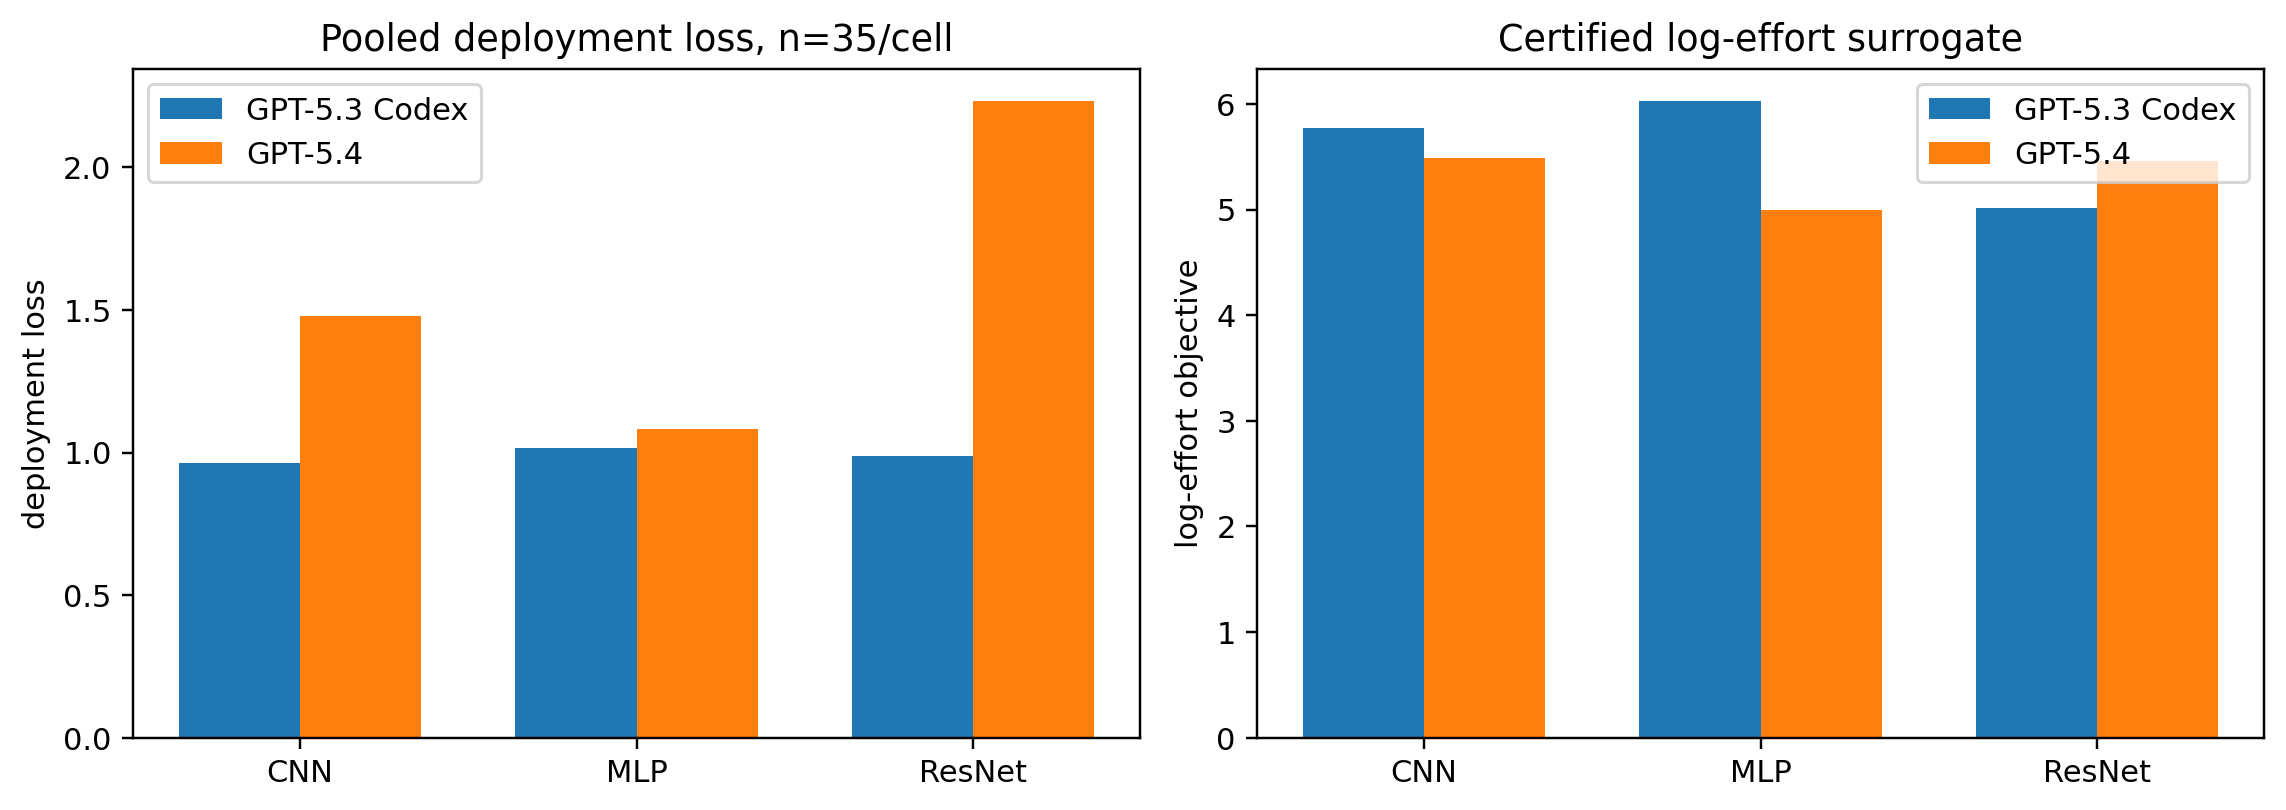
\includegraphics[width=\linewidth]{figures/autoresearch/twomodel_deployment_frontier.png}
\caption{Two-worker frontier on the 35-run pooled panel.
Left: first-passage deployment loss, lower is better.
Right: certified log-effort surrogate.
The two summaries disagree by mode: \texttt{gpt\_5\_4} reaches the threshold faster and has higher final verified improvement, while deployment-loss accounting favors \texttt{gpt\_5\_3\_codex} in the promoted two-worker panel.}
\label{fig:twomodel-frontier}
\end{figure}

\begin{table}[t]
\centering
\small
\caption{Different summaries select different workers on the same trajectories.
Speed uses lower mean first-hit step; quality uses higher final relative improvement; lower is better for log-effort and deployment loss.}
\label{tab:ranking-disagreement}
\begin{tabular}{@{}lccc@{}}
\toprule
Criterion & \textit{MLP-flat} & \textit{compact CNN} & \textit{micro ResNet} \\
\midrule
First-hit speed & \texttt{gpt\_5\_4} & \texttt{gpt\_5\_4} & \texttt{gpt\_5\_4} \\
Final improvement & \texttt{gpt\_5\_4} & \texttt{gpt\_5\_4} & \texttt{gpt\_5\_4} \\
Certified log-effort & \texttt{gpt\_5\_4} & \texttt{gpt\_5\_4} & \texttt{gpt\_5\_3\_codex} \\
Deployment loss & \texttt{gpt\_5\_3\_codex} & \texttt{gpt\_5\_3\_codex} & \texttt{gpt\_5\_3\_codex} \\
\bottomrule
\end{tabular}
\end{table}

The frontier already rejects a single leaderboard ordering.
Averaged across modes, \texttt{gpt\_5\_4} has lower mean first-hit step (2.45 vs.\ 5.35), higher final improvement (0.309 vs.\ 0.206), and lower mean log-effort (5.315 vs.\ 5.606).
Under the declared deployment loss, however, always using \texttt{gpt\_5\_3\_codex} has lower mean loss than always using \texttt{gpt\_5\_4} (0.989 vs.\ 1.598), and deployment-loss accounting selects \texttt{gpt\_5\_3\_codex} in all three modes.
Table~\ref{tab:ranking-disagreement} makes the mismatch explicit: conventional speed and quality favor \texttt{gpt\_5\_4}, the certified log-effort diagnostic is mode-dependent, and the promoted deployment loss favors \texttt{gpt\_5\_3\_codex}.
This is the empirical role of the decomposition: it exposes whether apparent performance comes from first-passage competence, cost, or mode-specific comparative advantage before a deployment loss decides the recommendation.
Appendix~\ref{app:diagnostic-plots} provides the threshold sensitivity, trajectory-level progress, cost, token, and router-record diagnostics behind these aggregate summaries.

\paragraph{Experiment 2: Signal audit.}
We audit whether richer pre-deployment records change the deterministic router's decision state.
This is not an estimator of \(\MI(S;Z_j)\): a Shannon-information estimate would require a frozen finite representation or predictive model for the signal records.
In the current diagnostic, budget-only records recover the three task-mode labels at 0.349 accuracy, while probe-containing records recover them perfectly on the diagnostic set.
Thus the signals can expose mode structure; the remaining question is whether the router converts that structure into better actions.

\paragraph{Experiment 3: Routing shift and action-frontier regret.}
We measure this conversion with shift rate and action-frontier regret.
Shift rate is the fraction of modes for which the richer signal changes the selected worker; action-frontier regret scores the selected action against the mode-conditional frontier from Experiment 1.
Both diagnostics are defined in Appendix~\ref{app:experiment-details}.

\begin{figure}[t]
\centering
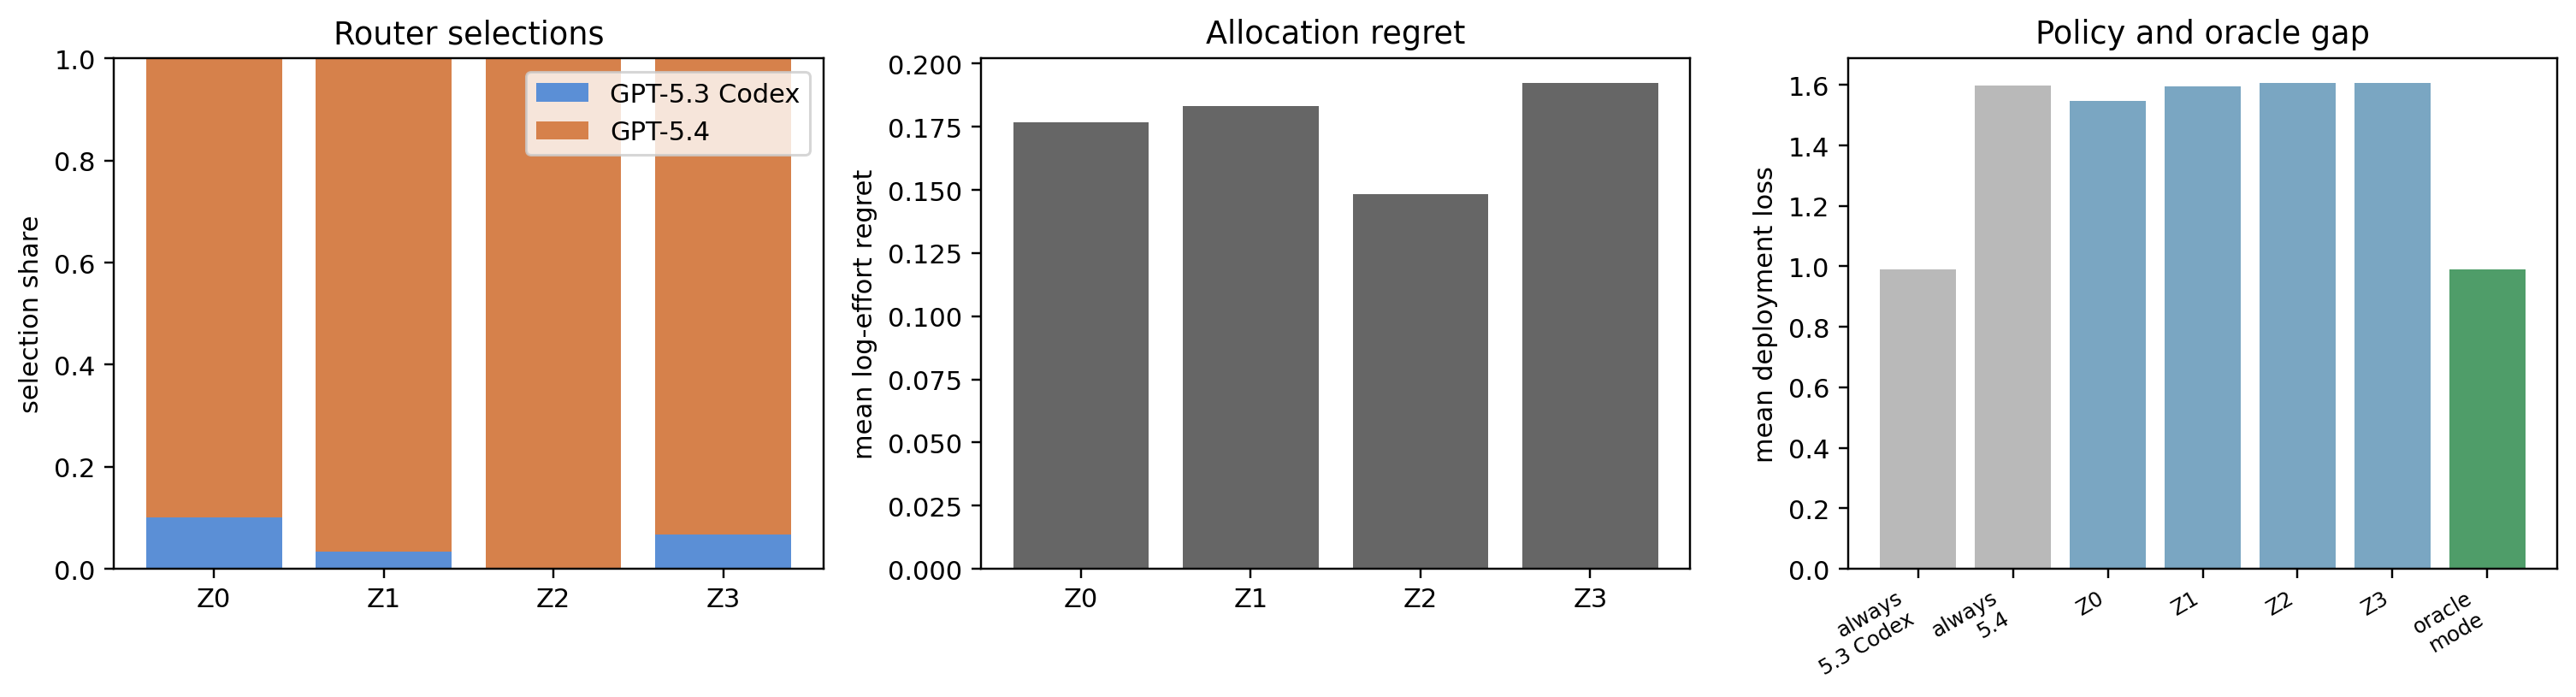
\includegraphics[width=\linewidth]{figures/autoresearch/twomodel_router_selection_regret.png}
\caption{Two-worker router-response audit.
Left: selected-worker distribution under real signal records.
Middle: action-frontier regret against the 35-run pooled log-effort frontier.
Right: deployment loss for always-worker baselines, prompt-router policies, and the mode oracle; under the primary loss the oracle coincides with always \texttt{gpt\_5\_3\_codex}.
Richer records expose mode information but do not reliably move the prompt-only router toward the deployment-loss recommendation.}
\label{fig:twomodel-router-regret}
\end{figure}

The final audit contains 480 prompt-only decisions.
On real signal records, the router remains strongly biased toward \texttt{gpt\_5\_4}.
Mean log-effort regret is 0.177 for \(Z_0\), 0.183 for \(Z_1\), 0.148 for \(Z_2\), and 0.192 for \(Z_3\).
Under the primary deployment loss, the non-deployable mode oracle in Figure~\ref{fig:twomodel-router-regret} coincides with always using \texttt{gpt\_5\_3\_codex}.
This makes the failure sharper than missing a subtle switching rule: the prompt-only router remains biased toward \texttt{gpt\_5\_4}, the worker favored by speed and final-quality metrics rather than by the declared deployment loss.
Under log-effort, the frontier remains mode-dependent, with \texttt{gpt\_5\_4} favored on \textit{MLP-flat} and \textit{compact CNN} and \texttt{gpt\_5\_3\_codex} favored on \textit{micro ResNet}; the paired deployment loss decides which diagnostic should govern the promoted recommendation.
Additional router-record completion and signal-ablation plots are reported in Appendix~\ref{app:diagnostic-plots}.

\paragraph{Experiment 4: Paired deployment gain.}
For each richer signal \(Z_j\), we compare the action selected under \(Z_j\) with the action selected under \(Z_0\) on the same executable-setting panel and subtract measurement cost:
\[
\widehat{\Delta}_R(j)=
\widehat{\ell}_{\mathrm{dep}}(\rho_0)-
\widehat{\ell}_{\mathrm{dep}}(\rho_j)-
\widehat{\ell}_{\mathrm{meas}}(j).
\]
Positive values mean that the richer signal improves net deployment loss after the cost of measuring or using the signal is charged.
This is the primary empirical estimand; positive signal information or lower regret alone is insufficient.

\begin{table}[t]
\centering
\small
\caption{Paired router validation on the final two-worker menu.
Net gain is \(\widehat{\ell}_{\mathrm{dep}}(\rho_0)-\widehat{\ell}_{\mathrm{dep}}(\rho_j)-\widehat{\ell}_{\mathrm{meas}}(j)\); positive is better.}
\label{tab:twomodel-router-gain}
\begin{tabular}{@{}lrrrrr@{}}
\toprule
Signal & Pairs & Shift & Gross gain & Meas. loss & Net gain \\
\midrule
\(Z_1\) & 30 & 0.133 & -0.049 & 0.000 & -0.049 \\
\(Z_2\) & 30 & 0.100 & -0.051 & 0.007 & -0.059 \\
\(Z_3\) & 30 & 0.100 & -0.032 & 0.028 & -0.060 \\
\bottomrule
\end{tabular}
\end{table}

The paired validation is negative for the current prompt-only router.
Against \(Z_0\), richer real signals produce small shift rates and negative net gain after measurement cost.
The bootstrap intervals from the accounting script are \([-0.116,0.002]\) for \(Z_1\), \([-0.127,-0.007]\) for \(Z_2\), and \([-0.113,-0.024]\) for \(Z_3\).
This is the main falsification result: informative records are not enough; the deployed router must use them in a way that improves the selected action's verified cost--success tradeoff.

\paragraph{Experiment 5: Negative controls.}
We repeat the router and paired-gain analyses with schema-preserving controls: shuffled probe records, wrong-mode probes, and synthetic noise records with matched field names and approximate context burden.
Controls are charged under the same measurement/context-cost convention as the corresponding real signal.
They test whether router response and paired gain are specific to task-relevant signal content.

The controls block a strong routing-information claim.
Wrong-mode \(Z_2\) has a small positive mean net gain with an interval crossing zero, while several shuffled or synthetic controls are negative with intervals similar to the real signals.
The correct conclusion is diagnostic rather than prescriptive: probes reveal task modes and the diagnostics expose ranking disagreement, but the primary deployment loss does not reward this router's action changes in the promoted two-worker menu.
Appendices~\ref{app:experiment-details} and~\ref{app:diagnostic-plots} state the full promotion rule and provide the negative-control figure used to separate diagnostic improvements from a deployable routing recommendation.

\section{Related work}
\label{sec:related}

The closest classical ancestor is algorithm selection.
Since Rice's formulation, solver portfolios have treated performance as instance-dependent: SATzilla and AutoFolio learn to select solvers from instance features rather than report one globally best solver~\citep{rice1976algorithm,xu2012satzilla,lindauer2015autofolio,kotthoff2016algorithm}.
Our contribution is the specialization to externally verified LLM agents, where a router observes a controlled pre-deployment record and is scored by paired deployment loss rather than standalone routing accuracy.
Unlike AutoML systems such as auto-sklearn, which tune pipelines offline for a dataset, our unit is a deployable action for a concrete verifier-backed instance~\citep{feurer2015autosklearn}.

LLM routing and cascades provide the model-menu context.
FrugalGPT, RouteLLM, RouterBench, LLMRouterBench, and compound-system routers study cost-quality routing over heterogeneous model pools~\citep{chen2023frugalgpt,ong2024routellm,hu2024routerbench,anonymous2026llmrouterbench,chen2025optimizing,yue2025masrouter,zaharia2024compound}.
We ask how much verified, task-specific information is worth before committing to an expensive agentic deployment.

verified agent benchmarks provide the task substrate.
SWE-bench evaluates repository repair against tests, AutoResearch evaluates training-loop edits against validation feedback, and theorem-proving systems use analogous external validators~\citep{jimenez2024swebench,karpathy2026autoresearch}.
Repeated sampling and inference-time scaling further show that lower-cost or smaller models can become competitive when verification is available~\citep{brown2024monkeys,snell2025testtime,wu2025inference,osca2024}.
Our question is upstream of the launched worker: which action should be selected, what should the router observe, and how should that observation be charged?

\section{Discussion and limitations}
\label{sec:discussion}

The paper separates a theory-facing diagnostic claim from a deployment-facing validation claim.
The experiments support the diagnostic claim: first-passage speed, final improvement, certified log-effort, and deployment loss disagree on the same verified task family.
They do not support the stronger claim that the evaluated prompt-only router improves deployment loss.
Probe records expose the predeclared task modes, but under the primary deployment loss the mature two-worker menu does not create a positive switching opportunity beyond always using \texttt{gpt\_5\_3\_codex}; the router remains biased toward the worker favored by speed and final-quality metrics.

The main limitations are the packed-mode abstraction, the fixed executable prototypes, and the two-worker mature action menu.
Real agent trajectories are stateful, task modes may be fuzzy, and the reported quantities are fixed-panel diagnostics rather than population-level deployment estimates.
This is why the appendix reports threshold curves, occupancy, cost sensitivity, token accounting, and signal-ablation checks instead of treating the finite-mode surrogate as sufficient.
The decomposition is therefore a claim discipline: it helps identify cost, competence, information, and allocation mechanisms, but paired deployment gain decides whether a routing recommendation is deployable.

\paragraph{Future work.}
The immediate experimental extension is to add a stable lower-cost action with matched trajectory support.
That would make the worker menu span a broader cost--capability frontier than the two-worker comparison reported here.
It would also test the retry-crossover theorem in its intended regime, where a lower-cost worker may compensate for lower one-attempt success through repeated verified attempts.
The ongoing \texttt{gpt\_5\_4\_mini} cells are not promoted here because support is still uneven across modes; they are the natural candidate for the retry-crossover experiment once matched at 35 trajectories per cell.
Beyond this benchmark, repository repair, theorem checking, and multi-file research-code editing would test less artificial mode schemas and more heterogeneous measurement costs.

\paragraph{Conclusion.}
Model choice inside an agent harness is not a scalar leaderboard problem.
It is a budget-aware deployment decision validated by paired outcomes after measurement cost.
The final two-worker study asks that question directly and answers it negatively for the current prompt-only router: pre-deployment information does not move allocation reliably enough to improve paired deployment loss.

\bibliographystyle{unsrtnat}
\bibliography{references}

\appendix


% ============================================================
% APPENDIX PATCH
% ============================================================

\section{Proofs: Certified-time derivation of log-effort}
\label{app:certified-log-effort}

This appendix derives the log-effort objective from certified time.
The main text uses only the certified-time definition, the coding-gain upper bound, and the
packed-mode identity.  Here we give the full chain:
\[
    \text{certified time}
    \;\longrightarrow\;
    \text{universal scheduling}
    \;\longrightarrow\;
    \text{coding-gain upper bound}
    \;\longrightarrow\;
    \text{packed latent-mode identity}
    \;\longrightarrow\;
    \text{finite-horizon empirical surrogate}.
\]

\subsection{Certified time and universal scheduling}

\paragraph{Verifiable task family.}
For each scale \(n\), let
\[
    \mathfrak T_n=(\cX_n,\cY_n,V_n,\mu_n)
\]
be a verifiable deployment task, where \(\cX_n\) is the instance space, \(\cY_n\) is the
artifact or solution space, \(V_n:\cX_n\times\cY_n\to\{0,1\}\) is an external verifier, and
\(\mu_n\) is the deployment distribution.
A randomized solver \(a\) maps \((x,r)\) to an artifact \(a(x;r)\), and its runtime is
\(\tau_a(x;r)\).

\begin{definition}[Certified time of a solver]
\label{def:app-certified-time}
For confidence level \(\delta_{\mathrm{cert}}\in(0,1)\), define
\[
    t_a(n,\delta_{\mathrm{cert}})
    :=
    \inf\left\{
        t>0:
        \Pr_{X\sim\mu_n,r}
        \big[
            V_n(X,a(X;r))=1
            \ \mathrm{and}\
            \tau_a(X;r)\le t
        \big]
        \ge 1-\delta_{\mathrm{cert}}
    \right\}.
\]
A solver is admissible at confidence \(\delta_{\mathrm{cert}}\) if this quantity is finite.
We write \(\cA_n^\delta\) for the admissible solver class.
\end{definition}

\paragraph{Prefix-coded schedules.}
Assume \(\cA_n^\delta\) is countable and prefix-coded.
A baseline universal scheduler assigns Kraft weights
\[
    \sum_{a\in\cA_n^\delta} w(a)\le 1,
\]
while a conditioned scheduler, after observing side information \(D\), assigns
\[
    \sum_{a\in\cA_n^\delta} w(a\mid D)\le 1.
\]
Giving solver \(a\) a share \(w(a)\) of wall-clock computation means that \(a\) receives
\(t_a\) internal units after approximately \(t_a/w(a)\) wall-clock units.  Thus the baseline
and conditioned certified times are
\[
    \overline T_U(n,\delta_{\mathrm{cert}})
    =
    c_{\mathrm{sim}}(n)
    \inf_{a\in\cA_n^\delta}
    \frac{t_a(n,\delta_{\mathrm{cert}})}{w(a)},
\]
and
\[
    \overline T_{U_D}(n,\delta_{\mathrm{cert}})
    =
    c_{\mathrm{sim}}(n)
    \inf_{a\in\cA_n^\delta}
    \frac{t_a(n,\delta_{\mathrm{cert}})}{w(a\mid D)}.
\]
Here \(c_{\mathrm{sim}}(n)\ge 1\) is a shared simulation overhead.

\begin{proposition}[Coding-gain bound]
\label{prop:app-coding-gain}
Fix a realization of \(D\), and let
\[
    a_D^\star
    \in
    \argmin_{a\in\cA_n^\delta}
    \frac{t_a(n,\delta_{\mathrm{cert}})}{w(a\mid D)}.
\]
Then
\[
    \log\frac{\overline T_U(n,\delta_{\mathrm{cert}})}
             {\overline T_{U_D}(n,\delta_{\mathrm{cert}})}
    \le
    \log\frac{w(a_D^\star\mid D)}{w(a_D^\star)}.
\]
\end{proposition}

\begin{proof}
By definition of \(a_D^\star\),
\[
    \overline T_{U_D}
    =
    c_{\mathrm{sim}}
    \frac{t_{a_D^\star}}{w(a_D^\star\mid D)}.
\]
Since \(\overline T_U\) is an infimum over all admissible solvers,
\[
    \overline T_U
    \le
    c_{\mathrm{sim}}
    \frac{t_{a_D^\star}}{w(a_D^\star)}.
\]
Dividing the two inequalities cancels both \(c_{\mathrm{sim}}\) and \(t_{a_D^\star}\), yielding
\[
    \frac{\overline T_U}{\overline T_{U_D}}
    \le
    \frac{w(a_D^\star\mid D)}{w(a_D^\star)}.
\]
Taking logs gives the claim.
\end{proof}

\paragraph{Interpretation.}
The bound says that side information cannot create certified speedup by magic.
It can only move scheduler mass toward a solver that is good for the realized problem.
On the log scale, this is a coding gain:
\[
    \log w(a\mid D)-\log w(a).
\]
This is the mathematical origin of the log objective.

\subsection{Resource-bounded information upper bound}

The coding-gain bound is pointwise and elementary.
To express it as an information upper bound, we need an aligned structure witness.
This subsection states a safe version with all assumptions explicit.

\begin{definition}[Resource-bounded structure length]
\label{def:app-ipoly}
Let \(H_n\) denote reusable task structure, and let
\[
    \cS(H_n)\subseteq\cA_n^\delta
\]
be a nonempty witness class of solvers realizing that structure.
Define
\[
    K^{\mathrm{poly}}(H_n)
    :=
    \inf_{a\in\cS(H_n)}\{-\log w(a)\},
\]
\[
    K^{\mathrm{poly}}(H_n\mid D)
    :=
    \inf_{a\in\cS(H_n)}\{-\log w(a\mid D)\},
\]
and
\[
    I_{\mathrm{poly}}(H_n:D)
    :=
    K^{\mathrm{poly}}(H_n)
    -
    K^{\mathrm{poly}}(H_n\mid D).
\]
\end{definition}

\begin{assumption}[Aligned witness]
\label{ass:app-aligned-witness}
For each realized \(D\), there exists a witness solver \(a_H(D)\in\cS(H_n)\) such that:
\[
    \log\frac{t_{a_H}}{w(a_H\mid D)}
    \le
    \inf_{a\in\cA_n^\delta}
    \log\frac{t_a}{w(a\mid D)}
    +
    \rho_D ,
\]
and
\[
    -\log w(a_H)
    \le
    K^{\mathrm{poly}}(H_n)+\kappa_D .
\]
The first inequality says the witness is nearly conditionally optimal.
The second says it is not much longer under the baseline code than the shortest solver
realizing the structure.
\end{assumption}

\begin{theorem}[Certified upper envelope]
\label{thm:app-certified-upper-envelope}
Under Assumption~\ref{ass:app-aligned-witness},
\[
    \log\frac{\overline T_U(n,\delta_{\mathrm{cert}})}
             {\overline T_{U_D}(n,\delta_{\mathrm{cert}})}
    \le
    I_{\mathrm{poly}}(H_n:D)+\kappa_D+\rho_D .
\]
If the overheads satisfy \(\kappa_D+\rho_D=O(\log n+\log\log(1/\delta_{\mathrm{cert}}))\),
then
\[
    \log\frac{\overline T_U(n,\delta_{\mathrm{cert}})}
             {\overline T_{U_D}(n,\delta_{\mathrm{cert}})}
    \le
    I_{\mathrm{poly}}(H_n:D)
    +
    O(\log n+\log\log(1/\delta_{\mathrm{cert}})).
\]
\end{theorem}

\begin{proof}
Let
\[
    L_U:=\inf_{a\in\cA_n^\delta}\left\{\log t_a-\log w(a)\right\},
    \qquad
    L_D:=\inf_{a\in\cA_n^\delta}\left\{\log t_a-\log w(a\mid D)\right\}.
\]
The shared simulation overhead cancels, so
\[
    \log\frac{\overline T_U}{\overline T_{U_D}}
    =
    L_U-L_D.
\]
For the aligned witness \(a_H=a_H(D)\),
\[
    L_U
    \le
    \log t_{a_H}-\log w(a_H),
\]
while Assumption~\ref{ass:app-aligned-witness} gives
\[
    L_D
    \ge
    \log t_{a_H}-\log w(a_H\mid D)-\rho_D.
\]
Therefore
\[
\begin{aligned}
    L_U-L_D
    &\le
    \bigl[\log t_{a_H}-\log w(a_H)\bigr]
    -
    \bigl[\log t_{a_H}-\log w(a_H\mid D)-\rho_D\bigr]
    \\
    &=
    -\log w(a_H)+\log w(a_H\mid D)+\rho_D.
\end{aligned}
\]
By the prior-length assumption,
\[
    -\log w(a_H)\le K^{\mathrm{poly}}(H_n)+\kappa_D.
\]
Since \(a_H\in\cS(H_n)\),
\[
    -\log w(a_H\mid D)\ge K^{\mathrm{poly}}(H_n\mid D),
\]
equivalently,
\[
    \log w(a_H\mid D)\le -K^{\mathrm{poly}}(H_n\mid D).
\]
Combining,
\[
    L_U-L_D
    \le
    K^{\mathrm{poly}}(H_n)-K^{\mathrm{poly}}(H_n\mid D)+\kappa_D+\rho_D
    =
    I_{\mathrm{poly}}(H_n:D)+\kappa_D+\rho_D .
\]
\end{proof}

\begin{remark}[Why the aligned-witness assumption is necessary]
The elementary coding-gain bound holds without a structure witness.
The \(I_{\mathrm{poly}}(H_n:D)\) upper bound does not.
It requires the solver accelerated by \(D\) to be a near-optimal representative of the
same reusable structure class \(H_n\).
Without this alignment, side information might favor a solver unrelated to the proposed
structure variable, and the claimed information upper bound would not follow.
\end{remark}

\subsection{Packed latent-mode family}

We now specialize the scheduler picture to the finite mode model used in the main text.

\begin{assumption}[Model-dependent packed latent-mode family]
\label{ass:app-packed-model}
Fix a task family and confidence level \(\delta_{\mathrm{cert}}\).
Assume:
\begin{enumerate}[leftmargin=1.25em,itemsep=0.15em]
    \item \textbf{Latent modes.}
    There is a finite latent mode
    \[
        S\in\cS=\{1,\ldots,m\},
        \qquad
        S\sim\pi.
    \]
    \item \textbf{Diagnostic signal.}
    A diagnostic signal \(D_M\) may depend on the model or harness \(M\), with posterior
    \[
        \pi_D^M(s):=\Pr[S=s\mid D_M=D].
    \]
    If the diagnostic is model-independent, we write simply \(D\) and \(\pi_D\).
    \item \textbf{Mode expert scale.}
    For each model/action \(M\) and mode \(s\), there is an internal certified scale
    \[
        t_0(M,s,\delta_{\mathrm{cert}})>0.
    \]
    \item \textbf{Cost.}
    Model/action \(M\) has per-unit deployment cost
    \[
        \kappa(M)>0.
    \]
    \item \textbf{Compute share.}
    After observing \(D\), the scheduler chooses a share vector
    \[
        q_D^M\in\Delta(\cS),
        \qquad
        \pi_D^M(s)>0\Rightarrow q_D^M(s)>0.
    \]
    \item \textbf{Inverse-share certified time.}
    Conditional on true mode \(s\), the certified time is
    \[
        \overline T^{(M)}_{q_D}(s,D)
        =
        c_{\mathrm{sim}}\,
        \kappa(M)\,
        \frac{t_0(M,s,\delta_{\mathrm{cert}})}{q_D^M(s)}.
    \]
\end{enumerate}
\end{assumption}

\paragraph{Why the inverse-share law is the right specialization.}
The universal scheduler gives solver \(a\) only a fraction \(w(a)\) of wall-clock computation,
so certified time is multiplied by \(1/w(a)\).
In the packed family, the finite dictionary of solvers is identified with the mode dictionary.
If the true mode is \(s\), only the share \(q_D^M(s)\) assigned to the correct mode expert
contributes to that expert's internal progress.
Thus assigning too little mass to the correct mode slows certified time by \(1/q_D^M(s)\).

\subsection{Conditional log-time decomposition}

\begin{lemma}[Conditional packed log-time]
\label{lem:app-conditional-packed}
Under Assumption~\ref{ass:app-packed-model}, for every realized \(D\),
\[
\begin{aligned}
    \E_{S\sim\pi_D^M}
    \bigl[
        \log \overline T^{(M)}_{q_D}(S,D)
    \bigr]
    &=
    \log c_{\mathrm{sim}}
    +
    \log\kappa(M)
    +
    \E_{S\sim\pi_D^M}
    [\log t_0(M,S,\delta_{\mathrm{cert}})]
    \\
    &\quad
    +
    H(\pi_D^M)
    +
    \KL(\pi_D^M\|q_D^M).
\end{aligned}
\]
For fixed \(M\) and \(D\), the unique minimizer over share vectors is
\[
    q_D^{M,\star}=\pi_D^M,
\]
on the support of \(\pi_D^M\), and the excess conditional expected log-time of any other
share vector is exactly
\[
    \KL(\pi_D^M\|q_D^M).
\]
\end{lemma}

\begin{proof}
From Assumption~\ref{ass:app-packed-model},
\[
    \log \overline T^{(M)}_{q_D}(s,D)
    =
    \log c_{\mathrm{sim}}
    +
    \log \kappa(M)
    +
    \log t_0(M,s,\delta_{\mathrm{cert}})
    -
    \log q_D^M(s).
\]
Taking expectation over \(S\sim\pi_D^M\), all terms are immediate except the last:
\[
    \E_{S\sim\pi_D^M}[-\log q_D^M(S)]
    =
    \sum_s \pi_D^M(s)\log\frac{1}{q_D^M(s)}.
\]
By the cross-entropy identity,
\[
    \sum_s \pi_D^M(s)\log\frac{1}{q_D^M(s)}
    =
    H(\pi_D^M)+\KL(\pi_D^M\|q_D^M).
\]
Nonnegativity of KL gives optimality, and equality holds only when
\(q_D^M=\pi_D^M\) on the support of \(\pi_D^M\).
\end{proof}

\subsection{Certified log-effort objective}

\begin{definition}[Packed certified log-effort]
\label{def:app-certified-log-effort}
For model/action \(M\) and allocation rule \(D\mapsto q_D^M\), define
\[
    \J_{\log}(M,q)
    :=
    \E_D
    \E_{S\sim\pi_D^M}
    \left[
        \log \overline T^{(M)}_{q_D}(S,D)
    \right]
    -
    \log c_{\mathrm{sim}}.
\]
Equivalently,
\[
\boxed{
    \J_{\log}(M,q)
    =
    \log\kappa(M)
    +
    \E_{S\sim\pi}
    [\log t_0(M,S,\delta_{\mathrm{cert}})]
    +
    \E_D
    \left[
        H(\pi_D^M)+\KL(\pi_D^M\|q_D^M)
    \right].
}
\]
Lower \(\J_{\log}\) means lower geometric-mean certified effort.
\end{definition}

\begin{proof}[Justification of the equivalent expression]
Apply Lemma~\ref{lem:app-conditional-packed} and average over \(D\).
The term
\[
    \E_D\E_{S\sim\pi_D^M}[\log t_0(M,S,\delta_{\mathrm{cert}})]
\]
equals
\[
    \E_{S\sim\pi}[\log t_0(M,S,\delta_{\mathrm{cert}})]
\]
by the tower property.
The shared \(\log c_{\mathrm{sim}}\) is subtracted by definition.
\end{proof}

\subsection{Routing-information identity}

The first identity holds model fixed and isolates information generation and routing mismatch.

\begin{theorem}[Routing-information identity]
\label{thm:app-routing-information}
Assume \(M\) is fixed, so \(t_0(M,s,\delta_{\mathrm{cert}})\) and \(\kappa(M)\) are common
to baseline and deployed systems.
Let the baseline use a fixed share vector \(q_0\), and let the deployed system use
\(D\mapsto q_D\).
Then
\[
\boxed{
    \E
    \left[
        \log \overline T_{q_0}(S)
        -
        \log \overline T_{q_D}(S,D)
    \right]
    =
    I_\pi(S;D)+\KL(\pi\|q_0)-\E_D\KL(\pi_D\|q_D).
}
\]
In particular, if \(q_0=\pi\),
\[
    \E
    \left[
        \log \overline T_{\pi}(S)
        -
        \log \overline T_{q_D}(S,D)
    \right]
    =
    I_\pi(S;D)-\E_D\KL(\pi_D\|q_D).
\]
\end{theorem}

\begin{proof}
For the fixed baseline \(q_0\), Lemma~\ref{lem:app-conditional-packed} with no diagnostic
conditioning gives
\[
    \E[\log \overline T_{q_0}(S)]
    =
    \log c_{\mathrm{sim}}
    +
    \log\kappa(M)
    +
    \E_\pi[\log t_0(M,S)]
    +
    H(\pi)
    +
    \KL(\pi\|q_0).
\]
For the deployed scheduler,
\[
    \E[\log \overline T_{q_D}(S,D)]
    =
    \log c_{\mathrm{sim}}
    +
    \log\kappa(M)
    +
    \E_\pi[\log t_0(M,S)]
    +
    \E_D H(\pi_D)
    +
    \E_D\KL(\pi_D\|q_D).
\]
Subtracting cancels cost and internal scale, leaving
\[
    H(\pi)-\E_DH(\pi_D)+\KL(\pi\|q_0)-\E_D\KL(\pi_D\|q_D).
\]
Since
\[
    I_\pi(S;D)=H(\pi)-\E_DH(\pi_D),
\]
the result follows.
\end{proof}

\subsection{Model-aware decomposition}

The previous theorem holds model fixed.
The model-aware version adds cost and mode-conditioned competence.

\begin{theorem}[Model-aware packed decomposition]
\label{thm:app-model-aware}
Under Assumption~\ref{ass:app-packed-model}, compare a baseline \((M_0,q_0)\) with a
deployed system \((M,q_D^M)\).
Then
\[
\boxed{
\begin{aligned}
&\E\!\left[
    \log \overline T^{(M_0)}_{q_0}(S)
    -
    \log \overline T^{(M)}_{q_D}(S,D_M)
\right]
\\
&\qquad =
\underbrace{\log\frac{\kappa(M_0)}{\kappa(M)}}_{\mathrm{cost}}
+
\underbrace{
\E_\pi
\left[
    \log\frac{t_0(M_0,S,\delta_{\mathrm{cert}})}
              {t_0(M,S,\delta_{\mathrm{cert}})}
\right]
}_{\mathrm{competence}}
+
\underbrace{I_\pi(S;D_M)}_{\mathrm{routing\ information}}
+
\underbrace{\KL(\pi\|q_0)}_{\mathrm{baseline\ mismatch}}
-
\underbrace{\E_{D_M}\KL(\pi_{D_M}^M\|q_{D_M}^M)}_{\mathrm{routing\ mismatch}} .
\end{aligned}
}
\]
If \(q_0=\pi\), this reduces to the four-term identity in the main text.
\end{theorem}

\begin{proof}
For the baseline,
\[
\begin{aligned}
    \E[\log \overline T^{(M_0)}_{q_0}(S)]
    &=
    \log c_{\mathrm{sim}}
    +
    \log\kappa(M_0)
    +
    \E_\pi[\log t_0(M_0,S,\delta_{\mathrm{cert}})]
    \\
    &\quad
    +
    H(\pi)
    +
    \KL(\pi\|q_0).
\end{aligned}
\]
For the deployed system, Lemma~\ref{lem:app-conditional-packed} gives
\[
\begin{aligned}
    \E[\log \overline T^{(M)}_{q_D}(S,D_M)]
    &=
    \log c_{\mathrm{sim}}
    +
    \log\kappa(M)
    +
    \E_\pi[\log t_0(M,S,\delta_{\mathrm{cert}})]
    \\
    &\quad
    +
    \E_{D_M}H(\pi_{D_M}^M)
    +
    \E_{D_M}\KL(\pi_{D_M}^M\|q_{D_M}^M).
\end{aligned}
\]
Subtracting yields
\[
\begin{aligned}
&\log\frac{\kappa(M_0)}{\kappa(M)}
+
\E_\pi
\left[
    \log\frac{t_0(M_0,S,\delta_{\mathrm{cert}})}
              {t_0(M,S,\delta_{\mathrm{cert}})}
\right]
\\
&\quad+
H(\pi)-\E_{D_M}H(\pi_{D_M}^M)
+
\KL(\pi\|q_0)
-
\E_{D_M}\KL(\pi_{D_M}^M\|q_{D_M}^M).
\end{aligned}
\]
The entropy difference is \(I_\pi(S;D_M)\).
\end{proof}

\subsection{From internal certified scale to success probability}

The decomposition above is exact in terms of the certified internal scale
\(t_0(M,s,\delta_{\mathrm{cert}})\).
The simpler notation \(p_M(s)\) is a specialization.

\paragraph{Exact geometric-trials calculation.}
Suppose each unit attempt of model \(M\) on mode \(s\) succeeds independently with
probability \(p_M(s)\in(0,1)\), and each unit attempt has normalized duration \(u_M(s)\).
After \(N\) attempts, the success probability is
\[
    1-(1-p_M(s))^N.
\]
To achieve failure probability at most \(\delta_{\mathrm{cert}}\), it is enough and necessary that
\[
    N
    \ge
    \frac{\log \delta_{\mathrm{cert}}}{\log(1-p_M(s))}
    =
    \frac{\log(1/\delta_{\mathrm{cert}})}
         {-\log(1-p_M(s))}.
\]
Thus an exact geometric certified scale is
\[
    t_0(M,s,\delta_{\mathrm{cert}})
    =
    u_M(s)
    \left\lceil
    \frac{\log(1/\delta_{\mathrm{cert}})}
         {-\log(1-p_M(s))}
    \right\rceil .
\]

\paragraph{Hazard approximation.}
For small or moderate \(p_M(s)\),
\[
    -\log(1-p_M(s))=p_M(s)+O(p_M(s)^2),
\]
so
\[
    t_0(M,s,\delta_{\mathrm{cert}})
    \approx
    u_M(s)\frac{\log(1/\delta_{\mathrm{cert}})}{p_M(s)}.
\]
If unit duration \(u_M(s)\) is absorbed into \(\kappa(M)\) or into the empirical cost term,
then, up to constants independent of the design comparison,
\[
    \log t_0(M,s,\delta_{\mathrm{cert}})
    \equiv
    -\log p_M(s).
\]
This is the origin of the paper's cost-adjusted log-effort surrogate
\[
    \log\kappa(M)-\log p_M(s)-\log q_D(s).
\]

\begin{remark}[Use hazard rather than raw success probability when \(p\) is large]
When \(p_M(s)\) is not small, the exact geometric scale is controlled by
\[
    h_M(s):=-\log(1-p_M(s)),
\]
not by \(p_M(s)\) itself.
In that regime the exact competence term is
\[
    \E_\pi
    \left[
        \log\frac{h_M(S)}{h_{M_0}(S)}
    \right]
\]
up to unit-duration factors.
The simpler \(p_M(s)\) notation should be read as an effective certified hazard or
finite-horizon success-efficiency surrogate.
\end{remark}

\subsection{Finite-horizon empirical surrogate}

In AutoResearch-style experiments, the ideal geometric-trials model is only a motivating
limit.  We therefore estimate finite-horizon quantities directly.

\paragraph{First-hit probability and cost.}
For model/action \(M\), mode \(s\), and horizon \(H\), define
\[
    F_M(s,H):=\Pr(\tau_M\le H\mid S=s),
\]
where \(\tau_M\) is the first verified threshold crossing, and
\[
    C_M(s,H):=\E[C_{\tau_M\wedge H}\mid M,S=s].
\]
The theorem-facing empirical log-effort loss is
\[
    \ell_{\mathrm{hit}}(M,s;H)
    =
    \log C_M(s,H)-\log(F_M(s,H)\vee\alpha),
\]
where \(\alpha>0\) is a censoring floor.

\paragraph{Occupancy when first hits saturate.}
If first-hit success saturates, as in the current AutoResearch pilot, we also report a
persistence statistic
\[
    O_M^\delta(s,H)
    =
    \E\left[
        \frac1H\sum_{h=1}^H
        \one\{G_{M,h}\ge\delta\}
        \,\middle|\,
        M,S=s
    \right],
\]
and the corresponding operational loss
\[
    \ell_{\mathrm{occ}}(M,s;H)
    =
    \log C_M^H(s,H)-\log(O_M^\delta(s,H)\vee\alpha).
\]
Here \(C_M^H(s,H)\) is the full no-stop trajectory cost.
This occupancy loss is not the exact packed theorem; it is an AutoResearch-facing
deployment diagnostic for durable verified progress.

\paragraph{Metric guardrail.}
The exact theorem decomposes
\[
    \E[\log \overline T(S,D)].
\]
The finite-horizon empirical losses approximate the same cost-divided-by-verified-progress
principle, but they are not equal to a global certified quantile.
For that reason the main experiments should report:
\[
    \ell_{\mathrm{hit}},
    \qquad
    \ell_{\mathrm{occ}},
    \qquad
    survival/hazard curves,
    \qquad
    and\ tail\ diagnostics
\]
rather than treating any single surrogate as the whole deployment objective.

\subsection{Approximate packedness and residual term}

The packed identity is exact under the inverse-share time law.
Outside that law, the correct statement is an identity plus a residual.

\begin{assumption}[Approximate inverse-share log-linearity]
\label{ass:app-approx-log-linear}
Suppose
\[
\begin{aligned}
    \log \overline T^{(M)}_{q_D}(s,D)
    &=
    \log c_{\mathrm{sim}}
    +
    \log\kappa(M)
    +
    \log t_0(M,s,\delta_{\mathrm{cert}})
    -
    \log q_D^M(s)
    \\
    &\quad
    +
    r_M(s,D,q_D),
\end{aligned}
\]
where
\[
    |r_M(s,D,q_D)|\le \eta
\]
uniformly over the evaluated design family.
\end{assumption}

\begin{proposition}[Residual form of the decomposition]
\label{prop:app-residual-decomp}
Under Assumption~\ref{ass:app-approx-log-linear}, the model-aware decomposition becomes
\[
\begin{aligned}
&\E[
    \log \overline T^{(M_0)}_{q_0}(S)
    -
    \log \overline T^{(M)}_{q_D}(S,D_M)
]
\\
&\qquad =
\log\frac{\kappa(M_0)}{\kappa(M)}
+
\E_\pi
\left[
    \log\frac{t_0(M_0,S)}{t_0(M,S)}
\right]
+
I_\pi(S;D_M)
+
\KL(\pi\|q_0)
-
\E_{D_M}\KL(\pi_{D_M}^M\|q_{D_M}^M)
+
R,
\end{aligned}
\]
where
\[
    R
    =
    \E[r_{M_0}(S,q_0)-r_M(S,D_M,q_D)].
\]
If \(|r|\le\eta\), then
\[
    |R|\le 2\eta.
\]
\end{proposition}

\begin{proof}
Substitute the approximate log-linear expression into the proof of
Theorem~\ref{thm:app-model-aware}.  All ideal terms decompose as before; the only leftover
terms are the two residuals.  Uniform boundedness gives
\[
    |R|
    \le
    \E|r_{M_0}(S,q_0)|+\E|r_M(S,D_M,q_D)|
    \le 2\eta.
\]
\end{proof}

\paragraph{Empirical use.}
The residual plot
\[
    \widehat{\mathrm{Res}}(d)
    =
    \widehat J_{\mathrm{obs}}(d)-\widehat J_{\mathrm{acct}}(d)
\]
is the empirical test of approximate packedness.
Large structured residuals by mode, model, horizon, or router indicate that the finite-mode
inverse-share abstraction is missing an interaction.


\section{Operational diagnostics}
\label{subsec:bridge}

The identity above becomes useful only after each term is tied to quantities logged by the deployment protocol.
The verifier-facing progress process is the common object used to operationalize competence, cost, information, and allocation diagnostics.
Fix a horizon $H$ and a task-normalized verified progress process $G_t(a,x)\in[0,1]$ for action $a$ on instance $x$.
In the main experiment, the router acts once before deployment: after observing $Z$, it selects one action, and that action is used for the whole trajectory.
The success and cost diagnostics below are therefore trajectory-level quantities computed from the step-wise verifier trace.
For lower-is-better verifier losses, one admissible normalization is
\[
G_t(a,x)
=
\operatorname{clip}_{[0,1]}\!\left(
\frac{L_0(x)-L_t(a,x)}{|L_0(x)|+\eps_L}
\right),
\]
where $L_0(x)$ is the starting-artifact loss and $L_t(a,x)$ is the verified loss convention at step $t$.
Given a success threshold $\delta>0$,
\[
\tau_\delta(a,x)=\inf\{t\le H:G_t(a,x)\ge \delta\},
\qquad
F_\delta(a,x)=\one\{\tau_\delta(a,x)=\infty\}.
\]
We also log persistence through
\[
\Occ_{\delta,H}(a,x)=\frac{1}{H}\sum_{t=1}^H \one\{G_t(a,x)\ge \delta\}.
\]
The full-horizon audit loss used for persistence and final-quality checks is
\begin{equation}
\ell_{\mathrm{audit}}(a,x;\xi)
=
\ell_{\mathrm{dep}}(a,x;\xi)
+\alpha_{\mathrm{occ}}\bigl(1-\Occ_{\delta,H}(a,x;\xi)\bigr)
+\alpha_{\mathrm{qual}}\psi(G_H(a,x;\xi)),
\label{eq:audit-loss}
\end{equation}
where \(\alpha_{\mathrm{occ}}=\alpha_{\mathrm{qual}}=1\) and \(\psi(u)=1-u\) after clipping \(G_H\in[0,1]\).
It is an audit diagnostic, not the primary deployment loss.

\paragraph{Competence.}
The action competence component $p(a,s)$ is the first-success probability of action $a$ on task mode $s$:
\[
p(a,s)=\Prb[\tau_\delta(a,X)\le H\mid S=s].
\]
Thus $G_t$ is step-wise, but the policy competence term uses the probability that the worker selected by the router reaches the success threshold at least once before the horizon.
Cumulative progress and persistence are not substituted for $p(a,s)$ in the identity.
We log
\[
\bar G_a(s)=\E\!\left[\frac{1}{H}\sum_{t=1}^H G_t(a,X)\mid S=s\right]
\]
and $\Occ_{\delta,H}$ as secondary diagnostics, especially when first-hit success saturates or when partial progress is scientifically relevant.

\paragraph{Cost.}
The action cost component $\kappa(a,s)$ is kept separate from competence.
In the main protocol it is the normalized cost of deploying action $a$ on mode $s$ for the same trajectory convention used to define $p(a,s)$.
The routed-policy cost term averages this mode-conditional cost over the actions selected under $Z$.
The primary convention is cost accumulated until the first certified success or the horizon, $\tau_\delta\wedge H$.
We log
\[
C_\delta(a,x;\xi)
=
\lambda^\top
\bigl(
\widetilde T^{\mathrm{worker}}_{\tau_\delta\wedge H},
\widetilde C^{\mathrm{tok}}_{\tau_\delta\wedge H}
\bigr)(a,x;\xi),
\]
and report worker wall-clock cost as primary, with token count as a sensitivity analysis.
verifier runtime is logged for audit, but it is not part of $\kappa(a,s)$ unless the verifier protocol or verifier-call frequency differs across actions.

\paragraph{Routing information.}
The theorem term $\MI(S;Z)$ measures how much a router-visible signal $Z$ separates the predeclared task modes before deployment.
This does not mean that the evaluator already knows the best worker for each instance.
The evaluator knows only the candidate mode schema and can estimate whether $Z_j$ makes that schema more identifiable:
\[
\MI(S;Z_j\mid Z_0)=\Hent(S\mid Z_0)-\Hent(S\mid Z_j).
\]
The quantity is estimated only when a finite signal representation or calibrated predictive model for the signal records is predeclared.
Otherwise the paper reports signal summaries and router-response diagnostics instead of a Shannon mutual-information estimate.
It is a descriptive information diagnostic; its decision value is established only after action outcomes show that the modes predict different cost--success profiles.
The paired router experiment then checks whether higher-information signals actually change the selected action and improve first-passage deployment outcomes.

\paragraph{Allocation-summary mismatch and allocation regret.}
The theorem term $\E_Z\KL(\pi_Z\|q_Z)$ is defined only after the evaluator predeclares a reproducible construction of the evaluator-side mode summary $q_Z$.
Operationally, the router returns an action, not a mode label or distribution.
When no such $q_Z$ construction is frozen, the experiment reports allocation regret as a separate action-frontier diagnostic.
After deployment runs, the evaluator estimates the mode-conditional frontier
\[
a^\star(s)\in\argmin_{a\in\cA}\{\log\kappa(a,s)-\log p(a,s)\},
\]
or the statistically indistinguishable set of frontier actions.
For a selected action $a=\rho_j(x)$ and mode $s=\sigma(x)$, the corresponding allocation regret diagnostic is
\[
r_j(x)
=
\bigl[\log\kappa(a,s)-\log p(a,s)\bigr]
-
\min_{a'\in\cA}\bigl[\log\kappa(a',s)-\log p(a',s)\bigr].
\]
This regret is computed retrospectively on a diagnostic split and validated on holdout instances; it is not an oracle input to the router.
High information with high allocation regret means that the progressive signal exposed useful mode structure, but the induced action did not exploit the empirical cost--success frontier.

After these diagnostics are estimated, the experiment still reports the decision-facing first-passage deployment loss in~\eqref{eq:deployment-loss} as final validation.
The full-horizon audit loss in~\eqref{eq:audit-loss} is reported separately for persistence and final-quality checks.
These losses are not replacements for the theorem; they test whether designs favored or explained by the diagnostics improve the practical deployment objective.

\section{Progressive-signal decomposition}
\label{app:operational-decomp}

The main four-term identity compares a deployed design to a prior-matched baseline.
For the V3 router experiment, it is often useful to compare two progressive signal conditions for the same router.
Assume a finite task mode $S\in\cS$ and, for each signal condition $j$, the conditional mode distribution induced by the realized signal record
\[
\pi_j(s\mid Z_j)=\Prb[S=s\mid Z_j].
\]
The fixed orchestrator $R$ induces the routing policy $a_R^j(Z_j)=R(Z_j)$.
If an evaluator-side mode summary $q_R^j(\cdot\mid Z_j)\in\Delta(\cS)$ has been predeclared, define
\[
\mathcal E_R^j(s,Z_j)
=
\frac{\kappa(a_R^j(Z_j),s)}
{p(a_R^j(Z_j),s)\,q_R^j(s\mid Z_j)} .
\]
The log-effort gain of signal condition $Z_j$ over $Z_0$ is
\[
\Delta_R^{\log}(j)
:=
\E[
\log \mathcal E_R^0(S,Z_0)-\log \mathcal E_R^j(S,Z_j)
].
\]
Expanding the cross-entropy terms gives
\[
\Delta_R^{\log}(j)
=
C_R(j)+\Phi_R(j)+G(j)+M_R(j),
\]
where
\begin{align*}
C_R(j)
&=
\E\!\left[
\log\frac{\kappa(a_R^0(Z_0),S)}{\kappa(a_R^j(Z_j),S)}
\right],
\\
\Phi_R(j)
&=
\E\!\left[
\log\frac{p(a_R^j(Z_j),S)}{p(a_R^0(Z_0),S)}
\right],
\\
G(j)
&=
\Hent(S\mid Z_0)-\Hent(S\mid Z_j),
\\
M_R(j)
&=
\E\!\left[
\KL(\pi_0(\cdot\mid Z_0)\|q_R^0(\cdot\mid Z_0))
-
\KL(\pi_j(\cdot\mid Z_j)\|q_R^j(\cdot\mid Z_j))
\right].
\end{align*}
When $Z_j$ refines $Z_0$, $G(j)=\MI(S;Z_j\mid Z_0)$.
This signal-mode decomposition is theory-facing and excludes measurement cost unless such a term is added explicitly.
It is a diagnostic companion to the deployment-gain estimand~\eqref{eq:router-gain}, not a replacement for it.

\section{Full selection protocol and experimental configuration}
\label{app:experiment-details}

\begin{algorithm}[Theory-to-deployment selection protocol]
\label{alg:decomp-selection}
\begin{tabular}{@{}r p{0.86\linewidth}@{}}
\textit{Input:} &
Task family, verifier, finite task-mode schema $\cS$, action menu $\cA$, admissible progressive signals $\{Z_j\}$, pilot cell count $n_{\mathrm{cell}}$, deployment repeats $Q_{\mathrm{dep}}$, confirmation budget.\\[0.25em]
\textit{Output:} &
Recommended signal-conditioned deployment policy, reported accounting terms, paired deployment gain, and calibration diagnostics.\\[0.35em]
1 &
\textit{Freeze the modes and loss.} Declare $\cS$, success threshold $\delta$, horizon $H$, cost normalizers, deployment loss~\eqref{eq:deployment-loss}, measurement costs, and router output contract.\\
2 &
\textit{Structured pilot.} For each action $a\in\cA$ and mode $s\in\cS$, estimate $\hat p(a,s)$, $\hat\kappa(a,s)$, first-hit curves, occupancy, and uncertainty intervals.\\
3 &
\textit{Signal and router diagnostics.} For each progressive signal $Z_j$, report any predeclared signal-information diagnostic and log the action allocation induced by the router.\\
4 &
\textit{Accounting score.} Compute the four log-effort terms from Theorem~\ref{thm:four-term} only for quantities whose diagnostic estimators were predeclared; otherwise report allocation regret separately.\\
5 &
\textit{Paired deployment validation.} On the same holdout instances, run the selected action under $Z_0$ and richer $Z_j$ conditions, score repeated selected-worker trajectories by~\eqref{eq:deployment-loss}, and subtract measurement cost.\\
6 &
\textit{Decision.} Choose the signal condition with the largest held-out $\widehat{\Delta}_R(j)$ subject to predeclared gates; use $\J$, frontier scores, and allocation regret as diagnostics, not as the final deployment objective.
\end{tabular}
\end{algorithm}

\paragraph{Panel of fixed executable settings.}
The main experiment is a repeated-trajectory panel of fixed executable settings rather than a population draw from \(\mu\).
Each task mode \(s\) is represented by one executable setting
\[
\chi_s=(A_s,D,\mathrm{split},u,\eta_s,V,B_V,H,\delta),
\]
where \(A_s\) is the editable \texttt{train.py} template and starting model class, \(D\) is CIFAR-10, \(\mathrm{split}\) is the fixed train/validation split, \(u\) is the model-initialization seed, \(\eta_s\) are starting optimization and architecture hyperparameters, \(V\) is the verifier, \(B_V\) is the verifier budget, \(H\) is the edit--verify horizon, and \(\delta\) is the success threshold.
Panel-level aggregates use \(\hat\pi(s)=1/3\).
The analyzed worker menu is \(\{\texttt{gpt\_5\_3\_codex},\texttt{gpt\_5\_4}\}\).
The paper-facing comparison sets \(\cA=\cM\): each deployable action is a single worker run under the common prompt and harness.

\paragraph{Task-mode construction.}
The paper-facing task modes are named by the starting model family in the editable artifact.
\textit{MLP-flat} (\texttt{mlp\_flat}) is a fully connected classifier over flattened CIFAR-10 inputs; \textit{compact CNN} (\texttt{cnn\_compact}) is a small convolutional classifier with local spatial inductive bias; and \textit{micro ResNet} (\texttt{resnet\_micro}) is a reduced residual convolutional classifier with skip connections.
They are not different datasets or different workers.
They are evaluator-defined variants of the same CIFAR-10 edit--verify task: the dataset, split, verifier, prompt harness, horizon, and success threshold are fixed, while the initial architecture family and associated template parameters change.
This choice makes the mode variable operationally meaningful for the theory, because different starting artifacts can change both first-passage competence \(p(a,s)\) and cost \(\kappa(a,s)\) for the same worker.

\paragraph{Progressive signal records.}
The router sees one of four nested pre-deployment records.
\(Z_0\) contains only the task name, verifier objective, worker menu, and budget.
\(Z_1\) adds the initial \texttt{train.py} plus a static workload summary: starting model class, parameter count, optimizer and budget settings, dataset/verifier identifiers, and parse/runtime availability.
\(Z_2\) adds a low-cost verifier probe of the unmodified artifact at a predeclared probe budget.
\(Z_3\) adds the full unmodified-artifact baseline under the deployment verifier budget.
Probe records include validation loss, validation accuracy, training seconds, total seconds, optimizer steps, parameter count, parse/runtime status, and probe budget.
Probe runs are outside the selected worker deployment: they are charged through \(\ell_{\mathrm{meas}}\) and do not consume the later deployment horizon or verifier budget.
The evaluator-only baseline used to compute \(G_t\) is router-visible only in \(Z_3\).

\paragraph{Experiment accounting.}
The worker frontier uses 35 trajectories per task-mode--worker cell.
The selected-router validation uses the same fixed panel and reports all richer signals \(j\in\{1,2,3\}\) rather than selecting a single best signal on the same data.
Negative controls keep the signal schema and approximate context burden of the matched real signal: shuffled probes, wrong-mode probes, and synthetic noise records are charged under the same measurement/context-cost convention as the real record they mimic.
For the router audit, the prompt-only router selects \texttt{gpt\_5\_4} on 27/30 budget-only records, 29/30 static-workload records, 30/30 probe records, and 28/30 full-scout records.

\paragraph{Promotion rule.}
A routing recommendation is promoted only when worker-frontier estimates, cost sensitivity, router shift, action-frontier regret, paired gain after measurement cost, and negative controls agree.
If diagnostics improve but paired deployment gain does not, the report treats the result as a mechanism failure rather than a useful router.

\begin{proposition}[Unbiased paired router-gain estimator]
\label{prop:paired-unbiased}
Assume task instances are sampled i.i.d.\ from $\mu$, the orchestrator, action menu, and signal protocols are fixed before evaluation, measurement costs are recorded without bias, and deployment seeds are independent conditional on selected action and instance.
The router is run once per instance and signal condition; the $Q_{\mathrm{dep}}$ deployment repeats estimate the conditional expected loss of the selected action.
For condition $j$, estimate
\[
\widehat{\Delta}_R(j)
=
\frac{1}{N}\sum_{i=1}^N
\left[
\frac{1}{Q_{\mathrm{dep}}}\sum_{q=1}^{Q_{\mathrm{dep}}}
\ell_{\mathrm{dep}}(a_{R,i}^0,x_i;\xi_{i,q}^{0})
-
\frac{1}{Q_{\mathrm{dep}}}\sum_{q=1}^{Q_{\mathrm{dep}}}
\ell_{\mathrm{dep}}(a_{R,i}^j,x_i;\xi_{i,q}^{j})
-
\widehat{\ell}_{\mathrm{meas}}(j,x_i)
\right].
\]
If the repeated-run averages are unbiased for the expected deployment losses of the selected actions, then
$\E[\widehat{\Delta}_R(j)]=\Delta_R(j)$.
\end{proposition}

When the same worker is selected under $Z_0$ and $Z_j$, using common deployment seeds preserves unbiasedness and reduces paired variance.
When counterfactual outcomes for all actions are logged on the same instance, hindsight action regret can be reported as a diagnostic, but it is not the primary estimand.
If the study fixes a finite panel of executable settings rather than sampling i.i.d.\ instances from $\mu$, the same estimator describes that panel and should not be interpreted as a population-level deployment estimand.

\begin{table}[t]
\centering
\small
\caption{Frozen operational configuration for the main protocol.
All values are fixed within a task mode; repeated runs vary only the agentic trajectory.}
\label{tab:train-config}
\begin{tabular}{@{}p{0.30\linewidth}p{0.60\linewidth}@{}}
\toprule
Component & Fixed value \\
\midrule
Dataset and split & CIFAR-10, $50{,}000$ training examples and $10{,}000$ validation examples; balanced subset, label noise $0.0$, imbalance ratio $1.0$; the train/validation split is fixed in the main protocol \\
Data seed & Common fixed data/subset seed; alternative split seeds are reported only as robustness variants \\
\texttt{train.py} initialization seed & \texttt{SEED=42}; used for Python, NumPy, PyTorch, CUDA seeds, deterministic PyTorch mode, and the training-loader generator; alternative initialization seeds are robustness variants \\
Training transforms & random crop with padding $4$, random horizontal flip, CIFAR-10 normalization; validation uses normalization only \\
Training budget per verifier call & fixed-step mode with \texttt{A\_MAX\_STEPS=256}; time budget \texttt{120s} is a fallback, not the primary scoring convention \\
Common hyperparameters & \texttt{BATCH\_SIZE=64}, \texttt{NUM\_WORKERS=0}, Adam, learning rate $5\cdot 10^{-4}$, weight decay $10^{-4}$, betas $(0.9,0.999)$, no LR schedule \\
Task mode & \textit{MLP-flat} (\texttt{mlp\_flat}), \textit{compact CNN} (\texttt{cnn\_compact}), or \textit{micro ResNet} (\texttt{resnet\_micro}) \\
Shared template parameters & depth $2$, base channels $12$, channel multiplier $2$, batch norm enabled, dropout $0.0$, and hidden width $48$ \\
Agent horizon & $H=20$ edit--verify steps; trajectories continue to $H$ after first success to measure persistence and final quality \\
Progress normalization & $\eps_L=10^{-8}$ in the denominator of $G_t$ \\
Primary loss weights & $\alpha_{\mathrm{fail}}=1$; normalized worker wall-clock is the primary scalar $C_\delta$; token cost is a sensitivity analysis \\
Audit loss weights & $\alpha_{\mathrm{occ}}=\alpha_{\mathrm{qual}}=1$, $\psi(u)=1-u$ \\
Measurement cost & pre-deployment probes are charged through $\ell_{\mathrm{meas}}$ using the same wall-clock normalizer as $C_\delta$; context-token cost is reported as sensitivity \\
Router configuration & deterministic prompt-only router with fixed model identifier, prompt hash, parser, temperature, top-p, and seed policy recorded before evaluation \\
\bottomrule
\end{tabular}
\end{table}

\paragraph{Trajectory record.}
Each run stores the worker alias, resolved model identifier, API date, split, task family, task mode, seed, maximum horizon $H$, signal condition, prompt hash, router model identifier, router temperature/top-p, router seed policy, parser version, router output, selected worker, and cost convention.
Each step stores the prompt-visible state, proposed \texttt{train.py} artifact, parse status, verifier result, validation loss, validation accuracy, relative improvement, incremental worker wall time, token usage, and verifier runtime for audit.
Parser failures are logged as unsuccessful routing or deployment records under the predeclared parser-failure policy.

\paragraph{Success and time-to-verification.}
For trajectory $i$, $\tau_i$ is the first step at which the relative improvement threshold is crossed; censored failures have $\tau_i=\infty$.
For each action-mode cell,
\[
  \hat F_a(s,h)=\frac{1}{n_{a,s}}\sum_i\one\{\tau_i\le h\},
  \qquad
  \hat S_a(s,h)=1-\hat F_a(s,h).
\]
The empirical hazard is
\[
  \hat\lambda_a(s,h)=
  \frac{\sum_i\one\{\tau_i=h\}}
       {\sum_i\one\{\tau_i\ge h\}} .
\]
The raw first-success estimate is $\hat p(a,s)=\hat F_a(s,H)$.
For log-effort scores, the protocol uses the predeclared smoothed estimate
\[
\tilde p(a,s)=\frac{k_{a,s}+1/2}{n_{a,s}+1},
\]
where $k_{a,s}$ is the number of first successes in the cell.
This prevents zero-success pilot cells from making log scores infinite; raw success counts are still reported.

\paragraph{Cost.}
The primary cost is cumulative worker wall-clock time to $\tau\wedge H$.
Secondary worker-side cost is cumulative token count.
verifier runtime is logged as a protocol audit field and excluded from action-cost comparisons unless the verifier protocol differs across actions.
All plots that support model recommendations must be reproducible under at least worker wall-clock and token-count conventions.
When a worker fails before producing a parseable artifact, its cost is still counted and the step is marked unsuccessful.
The scalar estimator matched to Assumption~\ref{ass:packed} is the cell mean
\[
\hat\kappa(a,s)=\frac{1}{n_{a,s}}\sum_{i:S_i=s} C_{\delta,i}(a),
\]
or its fixed-setting analogue $\hat\kappa_{\chi_s}(a)$ in Section~\ref{sec:experiments}.

\paragraph{Information, allocation summaries, and regret.}
For each progressive signal $Z_j$, a Shannon information estimate is reported only if the protocol predeclares a finite signal representation or calibrated predictive model for estimating $\pi_j(\cdot\mid Z_j)$ on held-out instances.
Otherwise the report uses qualitative signal summaries and router-response diagnostics without calling them estimates of $\MI(S;Z_j)$.
The KL mode-summary divergence term is reported only if the evaluator also freezes a reproducible construction of $\hat q_R^j(\cdot\mid Z_{j,i})$ before seeing evaluation outcomes.
For the deterministic router, the empirical panel shift rate is
\[
\widehat{\mathrm{Shift}}_R(j)=
\sum_{s\in\cS}\hat\pi(s)\one\{\rho_j(\chi_s)\ne\rho_0(\chi_s)\}.
\]
In the main fixed-setting protocol, the primary operational diagnostic is allocation regret,
\[
\hat r_j(x_i)
=
\bigl[\log\hat\kappa(a_{j,i},s_i)-\log\tilde p(a_{j,i},s_i)\bigr]
-
\min_{a\in\cA}
\bigl[\log\hat\kappa(a,s_i)-\log\tilde p(a,s_i)\bigr],
\]
where $a_{j,i}=R(Z_j(x_i))$ and $s_i=\sigma(x_i)$.

\paragraph{Uncertainty.}
Success probabilities use Wilson intervals.
Aggregated objectives, paired gains, and calibration diagnostics use bootstrap or randomization tests at the sampling unit declared for the study.
If the main protocol remains a panel of fixed executable settings, paired randomization tests over repeated trajectories are descriptive for that panel and should not be interpreted as population-level inference.
If independent task instances are added, uncertainty is reported at the task-instance level.

\section{Additional plots}
\label{app:diagnostic-plots}

This appendix collects auxiliary diagnostics generated from the experimental logs.
The threshold, trajectory, and cost diagnostics below use the same analyzed workers, \texttt{gpt\_5\_3\_codex} and \texttt{gpt\_5\_4}.
These appendix plots use the same 35-trajectory-per-cell panel as the main analysis.
The pooled appendix plots are robustness and mechanism diagnostics for the same accounting quantities reported in the main text.

\begin{table}[ht]
\centering
\small
\caption{Worker-frontier summary on the 35-run pooled panel.
Each cell uses 35 trajectories.
Lower is better for log-effort and deployment loss.}
\label{tab:twomodel-frontier}
\resizebox{\linewidth}{!}{%
\begin{tabular}{@{}llrrrr@{}}
\toprule
Mode & Worker & Success & Mean $\tau$ & Log-effort & Dep. loss \\
\midrule
\textit{MLP-flat} & \texttt{gpt\_5\_3\_codex} & 32/35 & 7.41 & 6.029 & 1.015 \\
\textit{MLP-flat} & \texttt{gpt\_5\_4} & 35/35 & 2.49 & 4.991 & 1.083 \\
\textit{compact CNN} & \texttt{gpt\_5\_3\_codex} & 34/35 & 6.03 & 5.774 & 0.964 \\
\textit{compact CNN} & \texttt{gpt\_5\_4} & 35/35 & 3.06 & 5.492 & 1.479 \\
\textit{micro ResNet} & \texttt{gpt\_5\_3\_codex} & 35/35 & 2.60 & 5.015 & 0.987 \\
\textit{micro ResNet} & \texttt{gpt\_5\_4} & 35/35 & 1.80 & 5.461 & 2.234 \\
\bottomrule
\end{tabular}}
\end{table}

\begin{figure}[ht]
\centering
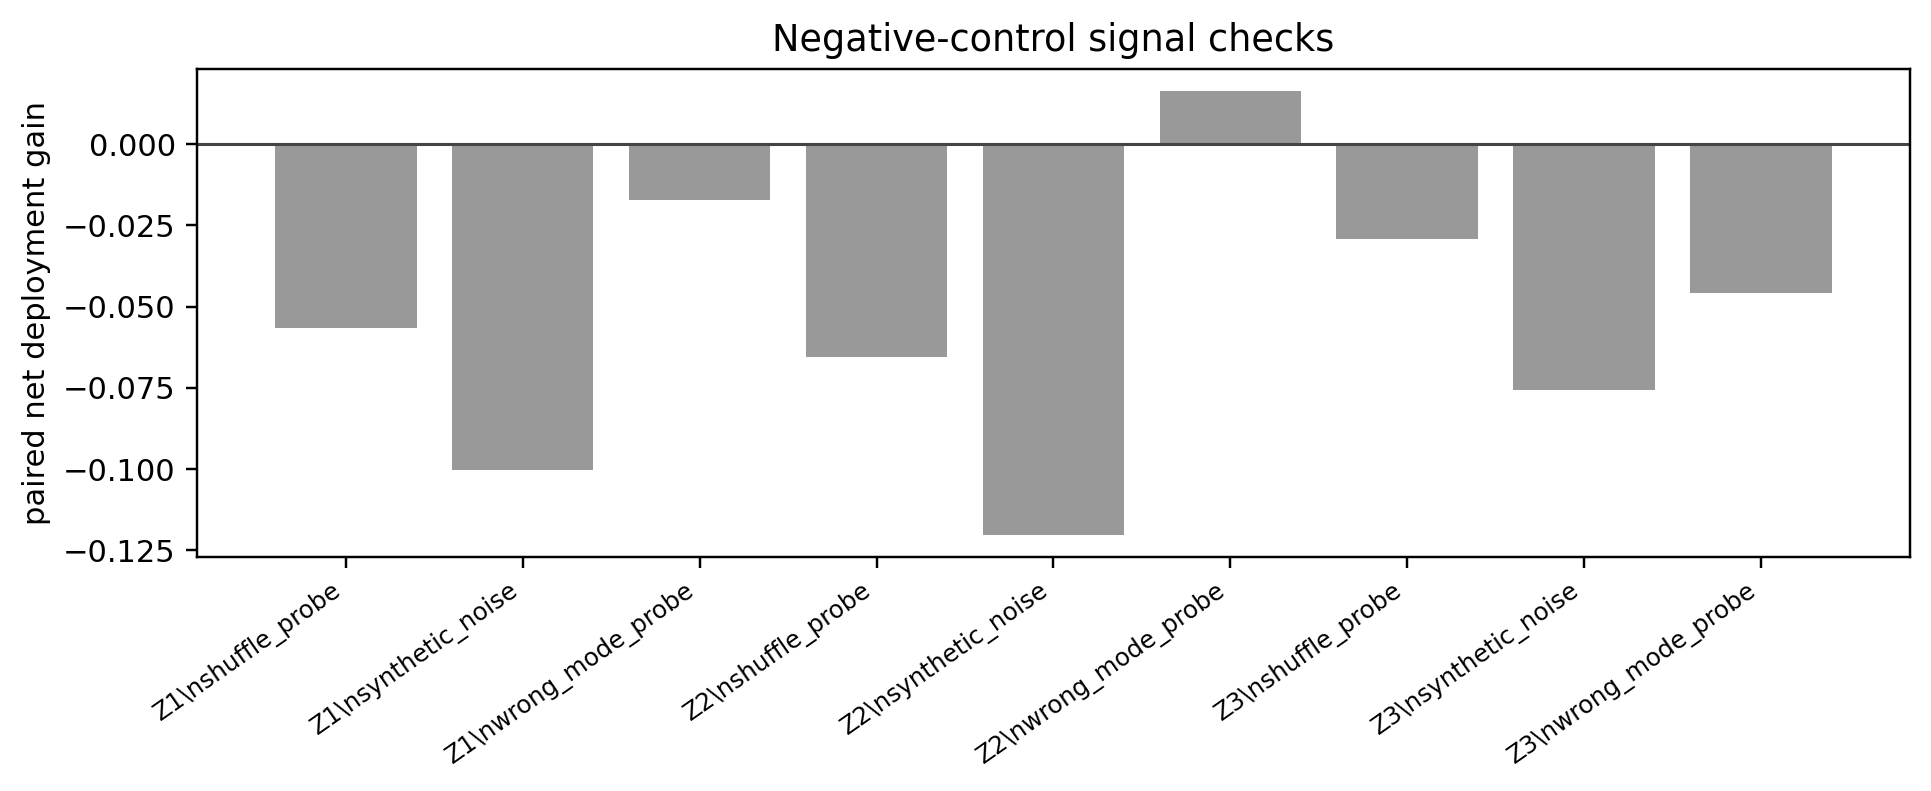
\includegraphics[width=\linewidth]{figures/autoresearch/twomodel_negative_controls.png}
\caption{Negative-control paired gains for shuffled probes, wrong-mode probes, and synthetic noise records.
The real records do not cleanly outperform the controls, indicating that the current prompt-only router is not reliably exploiting task-relevant measurement content.}
\label{fig:app-negative-controls}
\end{figure}

\subsection{Pooled threshold and trajectory diagnostics}
\label{app:pilot-threshold-diagnostics}

\begin{figure}[p]
\centering
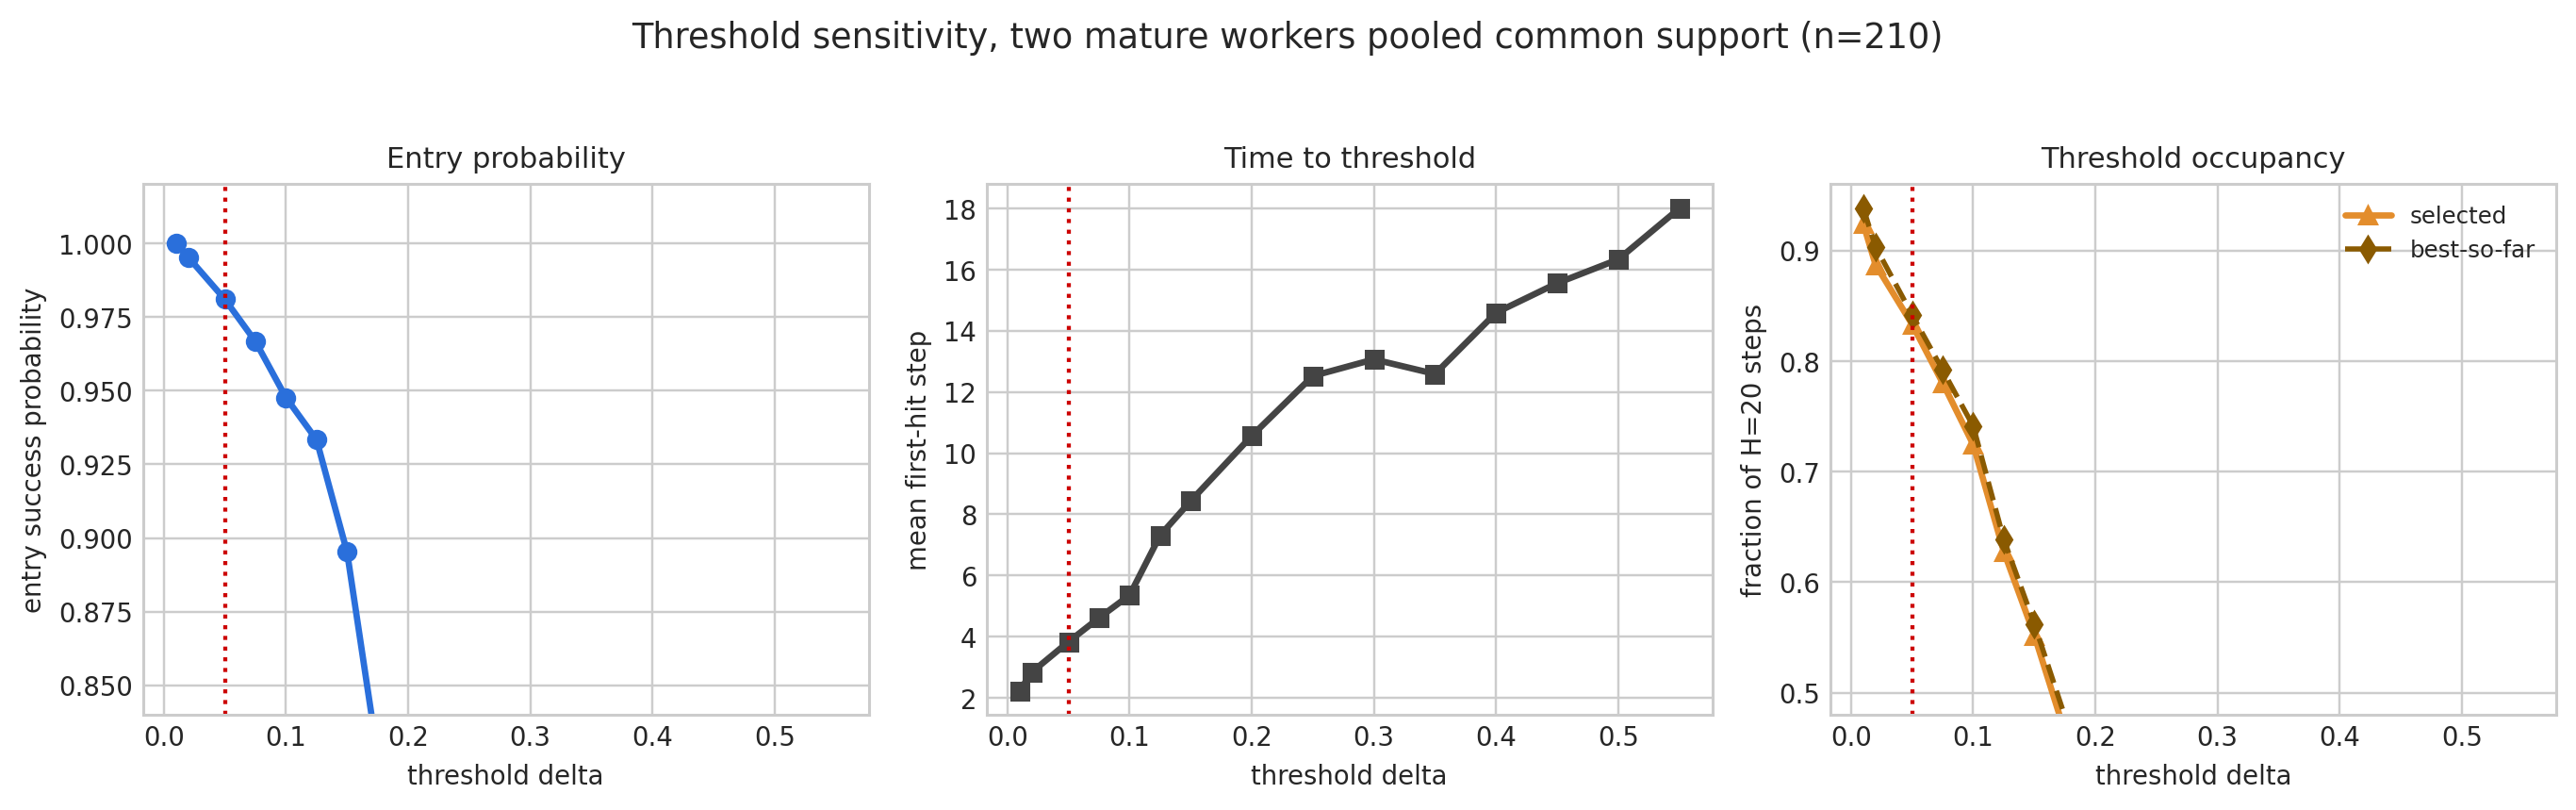
\includegraphics[width=\linewidth]{figures/autoresearch/diag_threshold_sensitivity_current_pilot.png}
\caption{Zoomed threshold sensitivity for the two mature workers on the 35-run pooled panel.
The red line marks the operating threshold \(\delta=0.05\).
At this threshold, entry success is near saturated while mean first-hit time remains low, which makes \(\delta=0.05\) a pragmatic operating point for studying time-to-certified-solution.
The sharp drop at larger thresholds shows why the exact threshold is not an innocuous plotting choice.}
\label{fig:app-threshold-sensitivity-zoom}
\end{figure}

\begin{figure}[p]
\centering
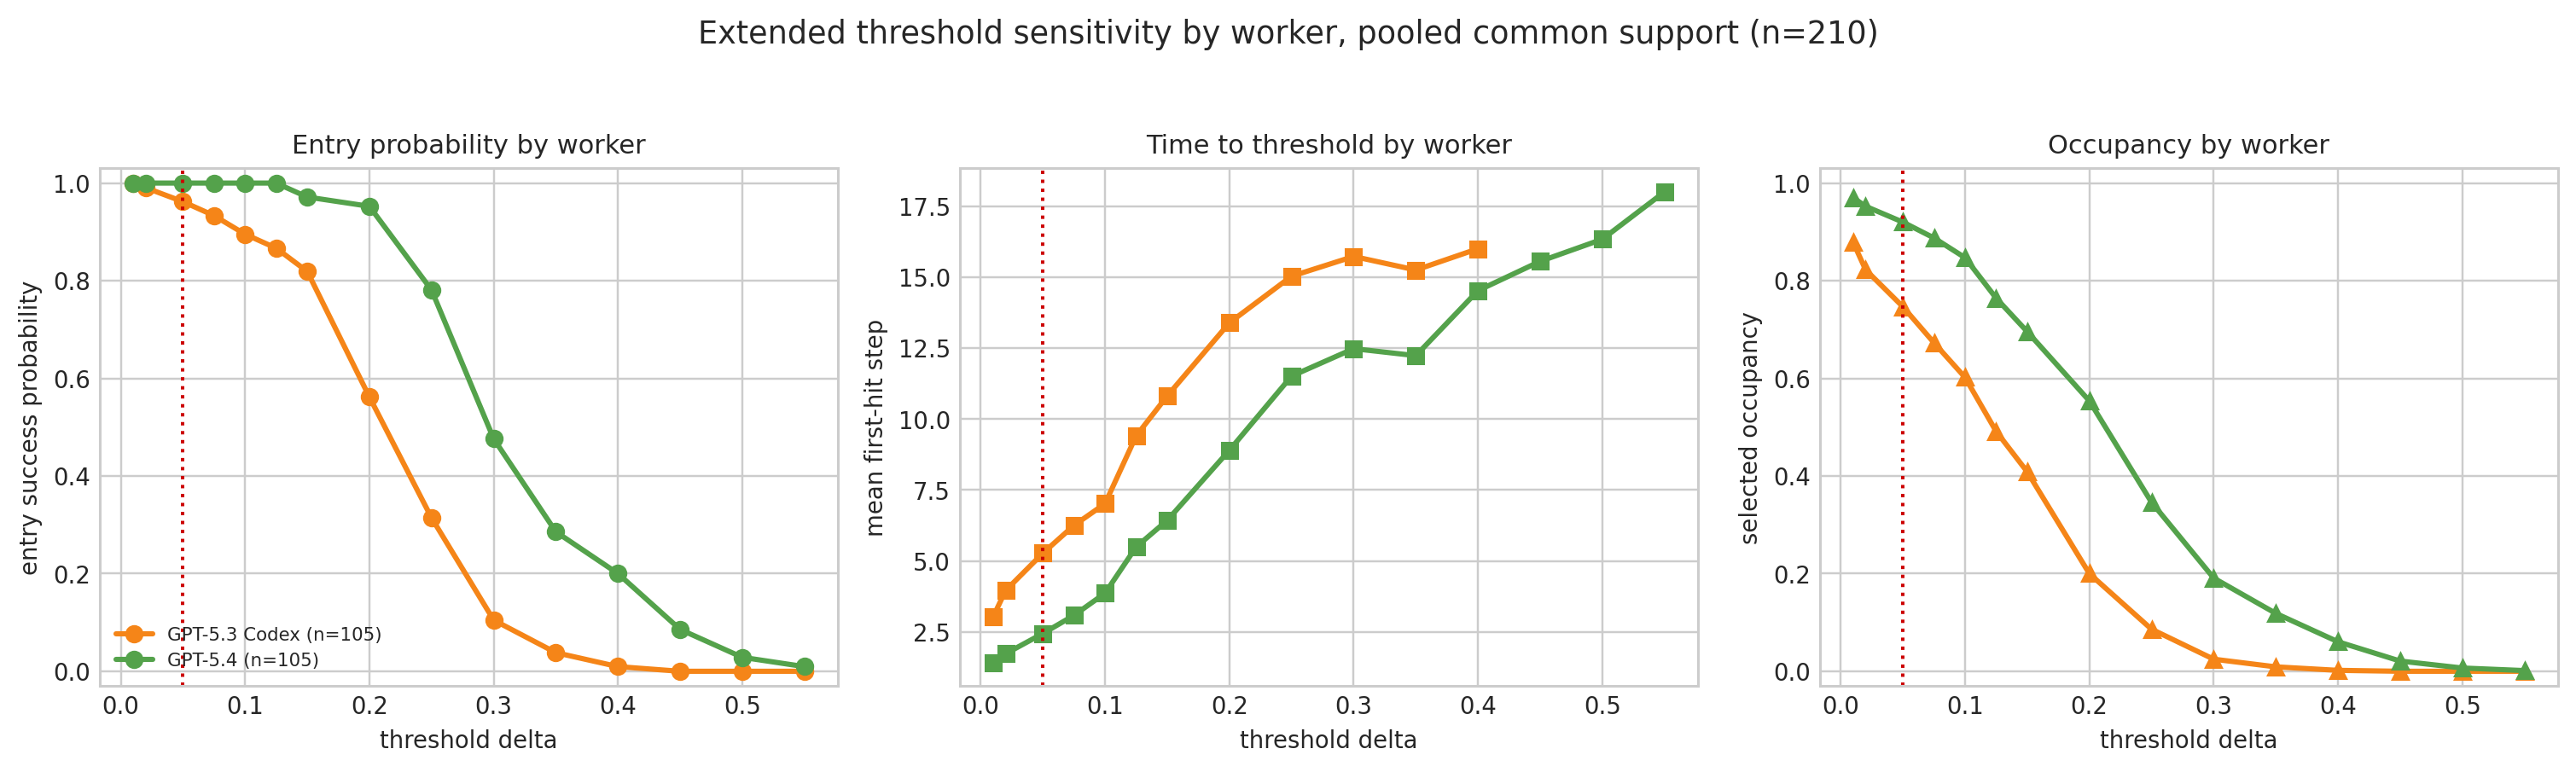
\includegraphics[width=\linewidth]{figures/autoresearch/diag_threshold_sensitivity_by_worker.png}
\caption{Threshold sensitivity by worker on the 35-run pooled panel.
\texttt{gpt\_5\_4} remains stronger at higher thresholds, while \texttt{gpt\_5\_3\_codex} degrades earlier; this supports the competence term in Theorem~\ref{thm:four-term}.}
\label{fig:app-threshold-by-worker}
\end{figure}

\begin{figure}[p]
\centering
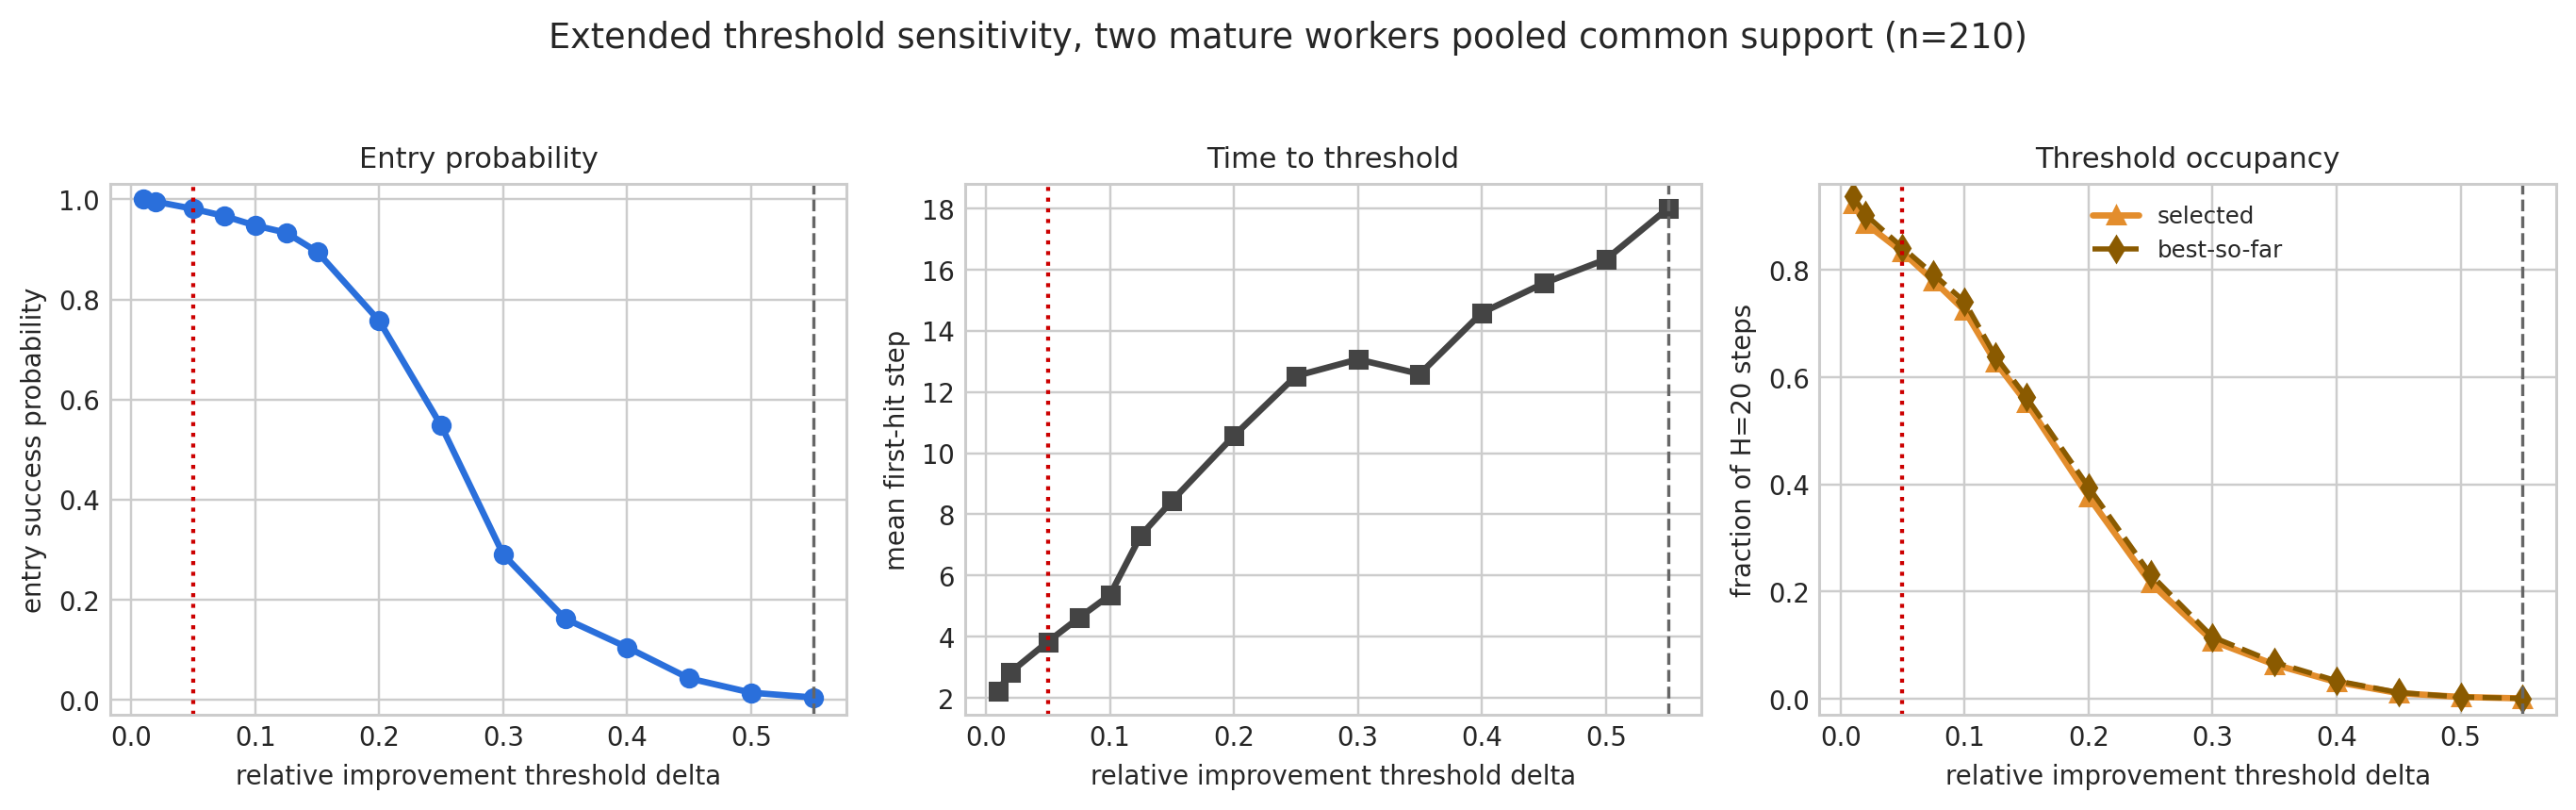
\includegraphics[width=\linewidth]{figures/autoresearch/diag_threshold_sensitivity_extended_current_pilot.png}
\caption{Extended threshold sensitivity for the two-worker pooled panel.
The full threshold range shows that high-threshold success is rare even when \(\delta=0.05\) is nearly saturated.
This is why the paper reports first-passage curves, occupancy, and final quality rather than relying on a single binary success rate.}
\label{fig:app-threshold-extended}
\end{figure}

\begin{figure}[p]
\centering
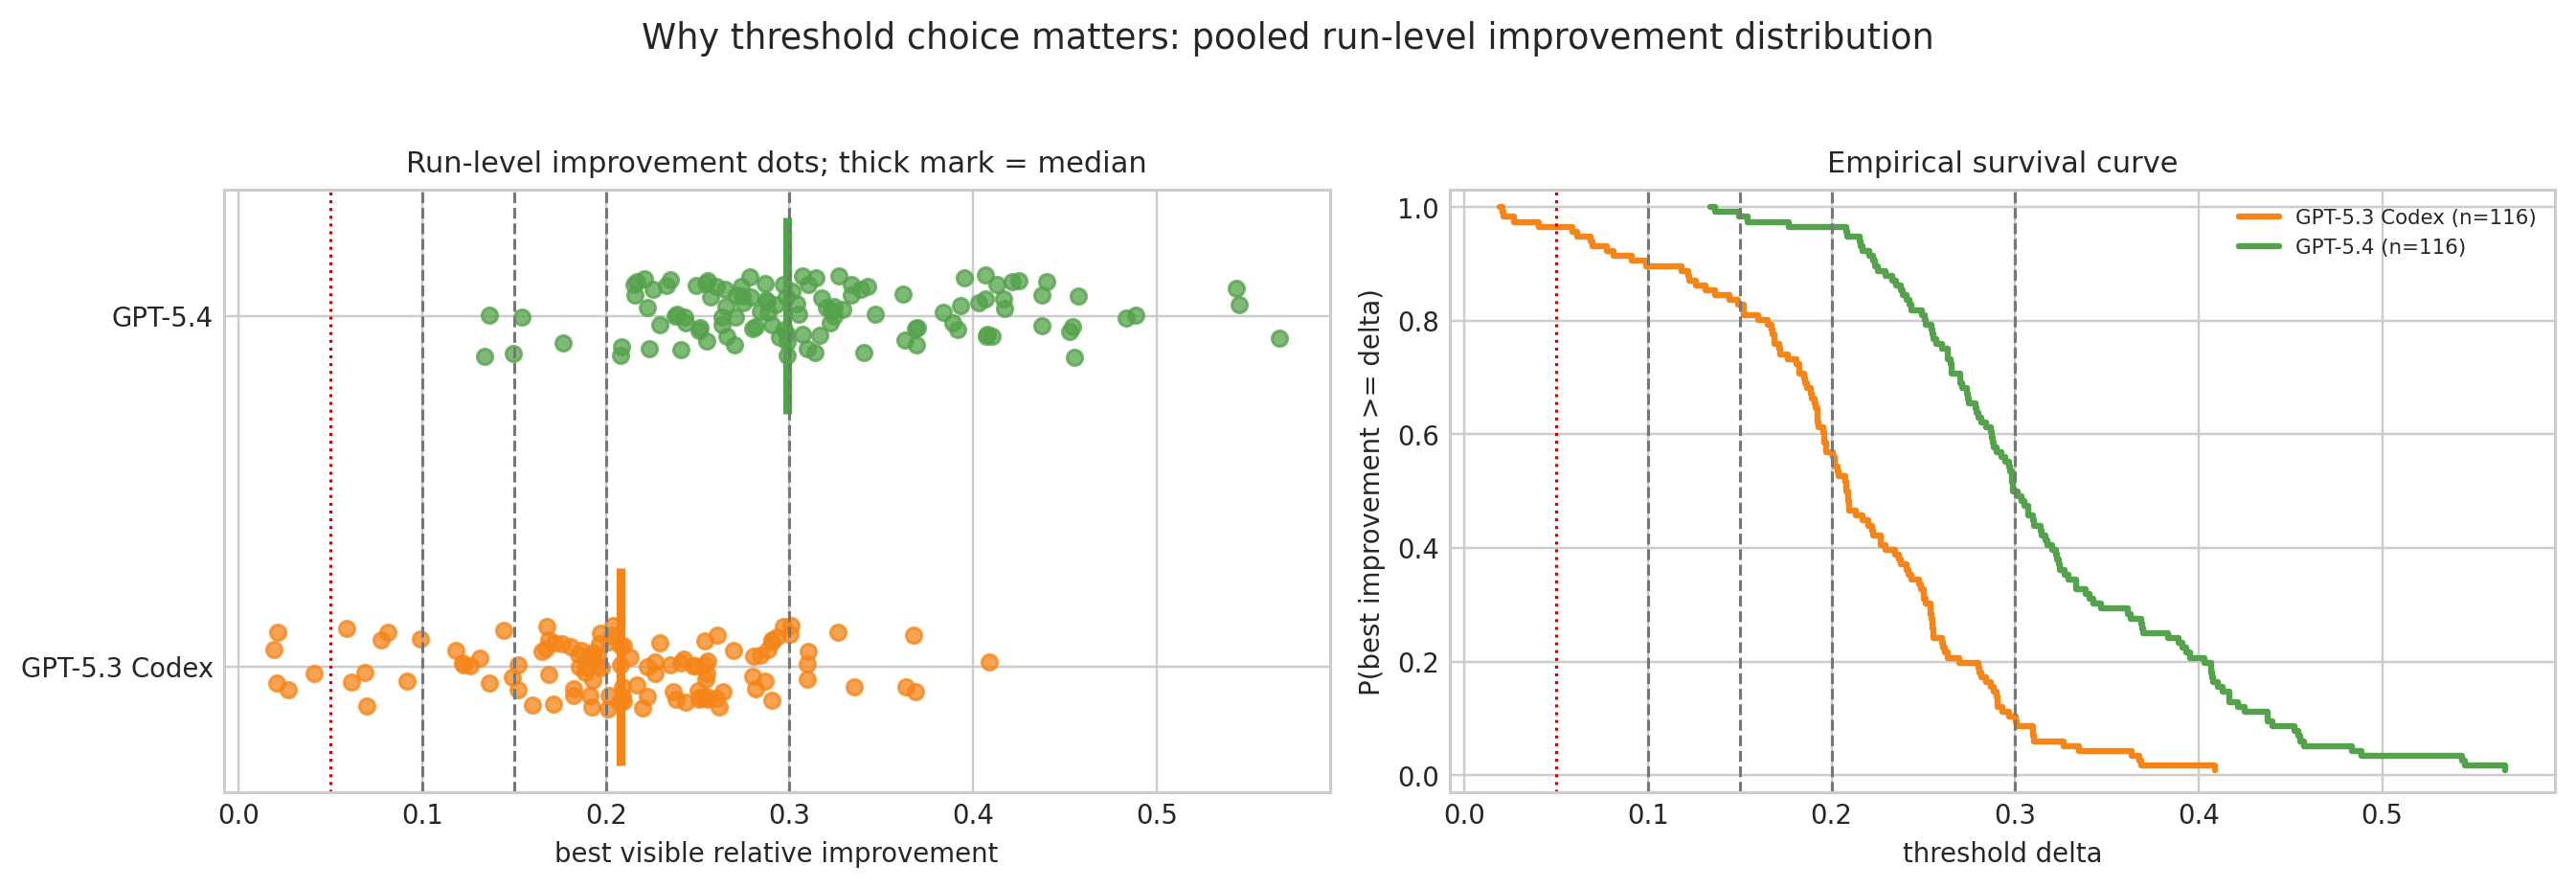
\includegraphics[width=\linewidth]{figures/autoresearch/diag_improvement_distribution_by_worker.png}
\caption{Run-level improvement distribution for the two mature workers.
Dots show final best-visible relative improvement and thick ticks mark worker medians.
The survival plot makes the threshold choice explicit: near \(\delta=0.05\), most runs succeed, but the ordering and separation change at higher thresholds.
This diagnostic supports the paper's claim that final quality, first-passage success, and deployment loss are distinct empirical objects.}
\label{fig:app-improvement-distribution}
\end{figure}

\begin{figure}[p]
\centering
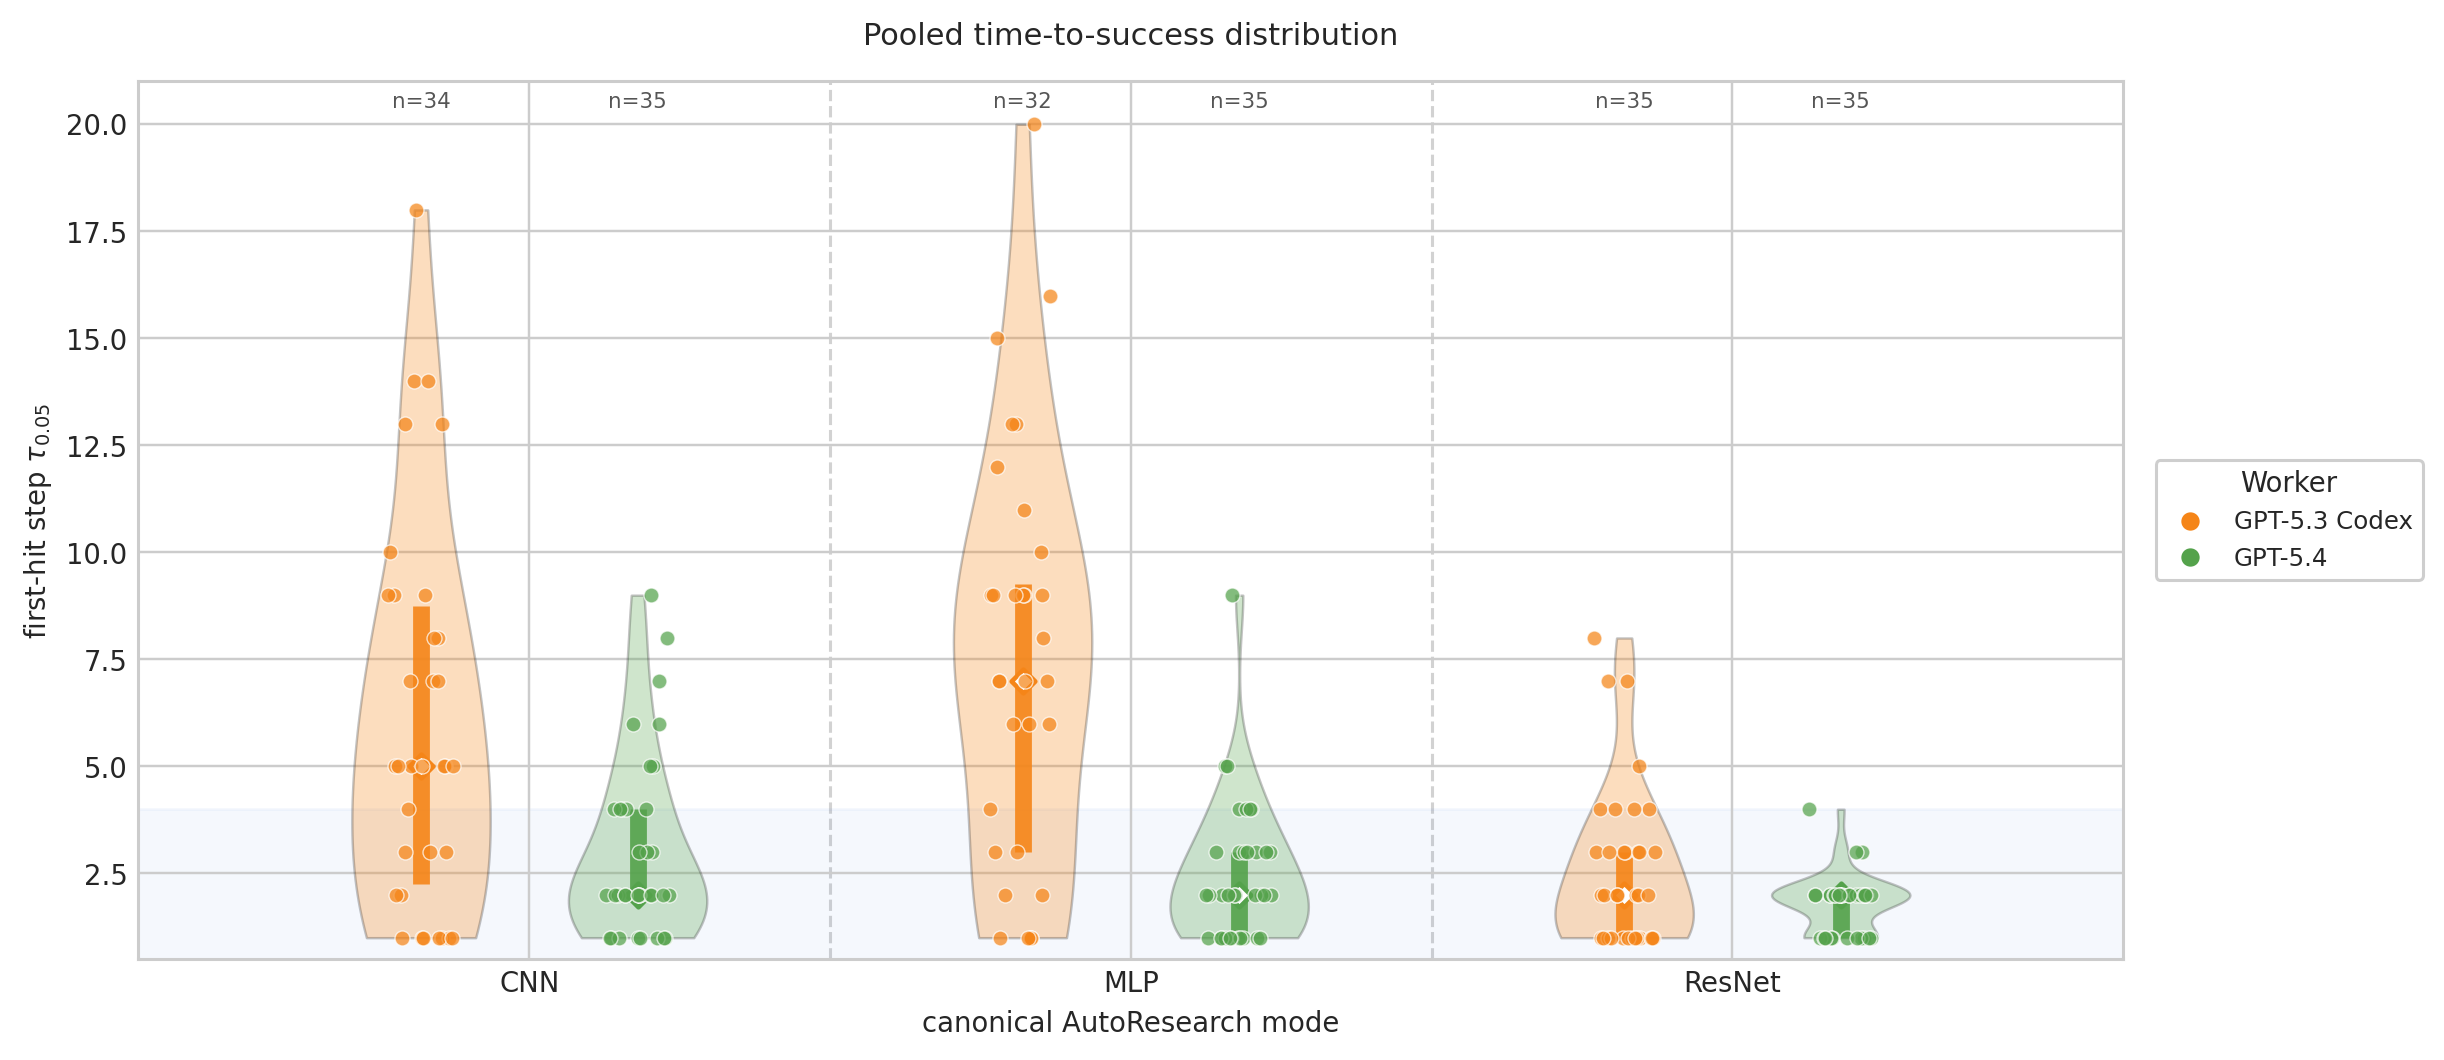
\includegraphics[width=\linewidth]{figures/autoresearch/diag_tau_distribution_pilot.png}
\caption{Pooled time-to-success distribution by task mode and worker.
The violin plots expose mode-conditional heterogeneity: \texttt{gpt\_5\_4} typically hits the threshold quickly, while \texttt{gpt\_5\_3\_codex} has broader first-hit times, especially on MLP.
This is the empirical object behind the cost and competence terms of the four-term decomposition.}
\label{fig:app-tau-distribution}
\end{figure}

\begin{figure}[p]
\centering
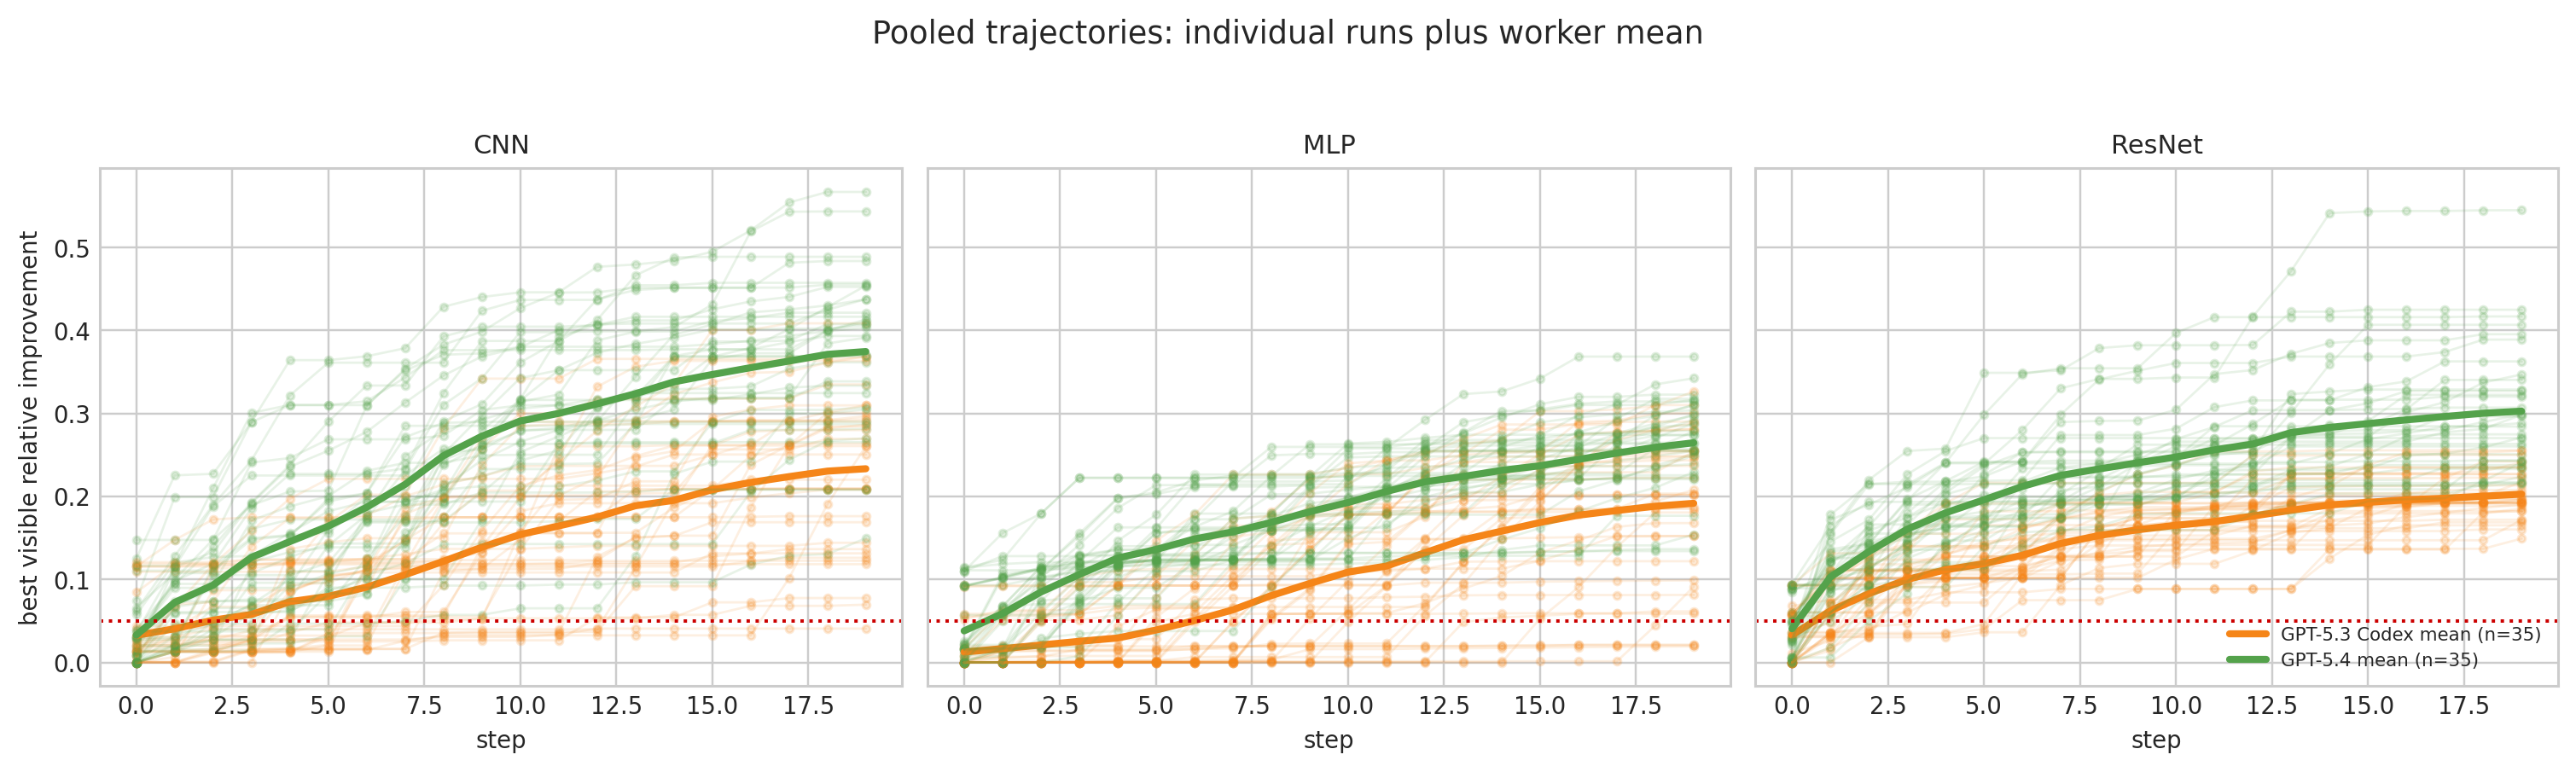
\includegraphics[width=\linewidth]{figures/autoresearch/diag_relative_improvement_spaghetti.png}
\caption{Best-so-far improvement trajectories.
The mean trajectories show that \texttt{gpt\_5\_4} improves earlier and reaches higher final relative improvement in the pooled panel, but the deployment accounting in the main text shows that this does not automatically imply lower deployment loss after cost is charged.
This contrast is the main empirical reason to separate worker competence from deployment value.}
\label{fig:app-improvement-trajectories}
\end{figure}

\subsection{Pooled cost diagnostics}
\label{app:pilot-cost-diagnostics}

\begin{figure}[p]
\centering
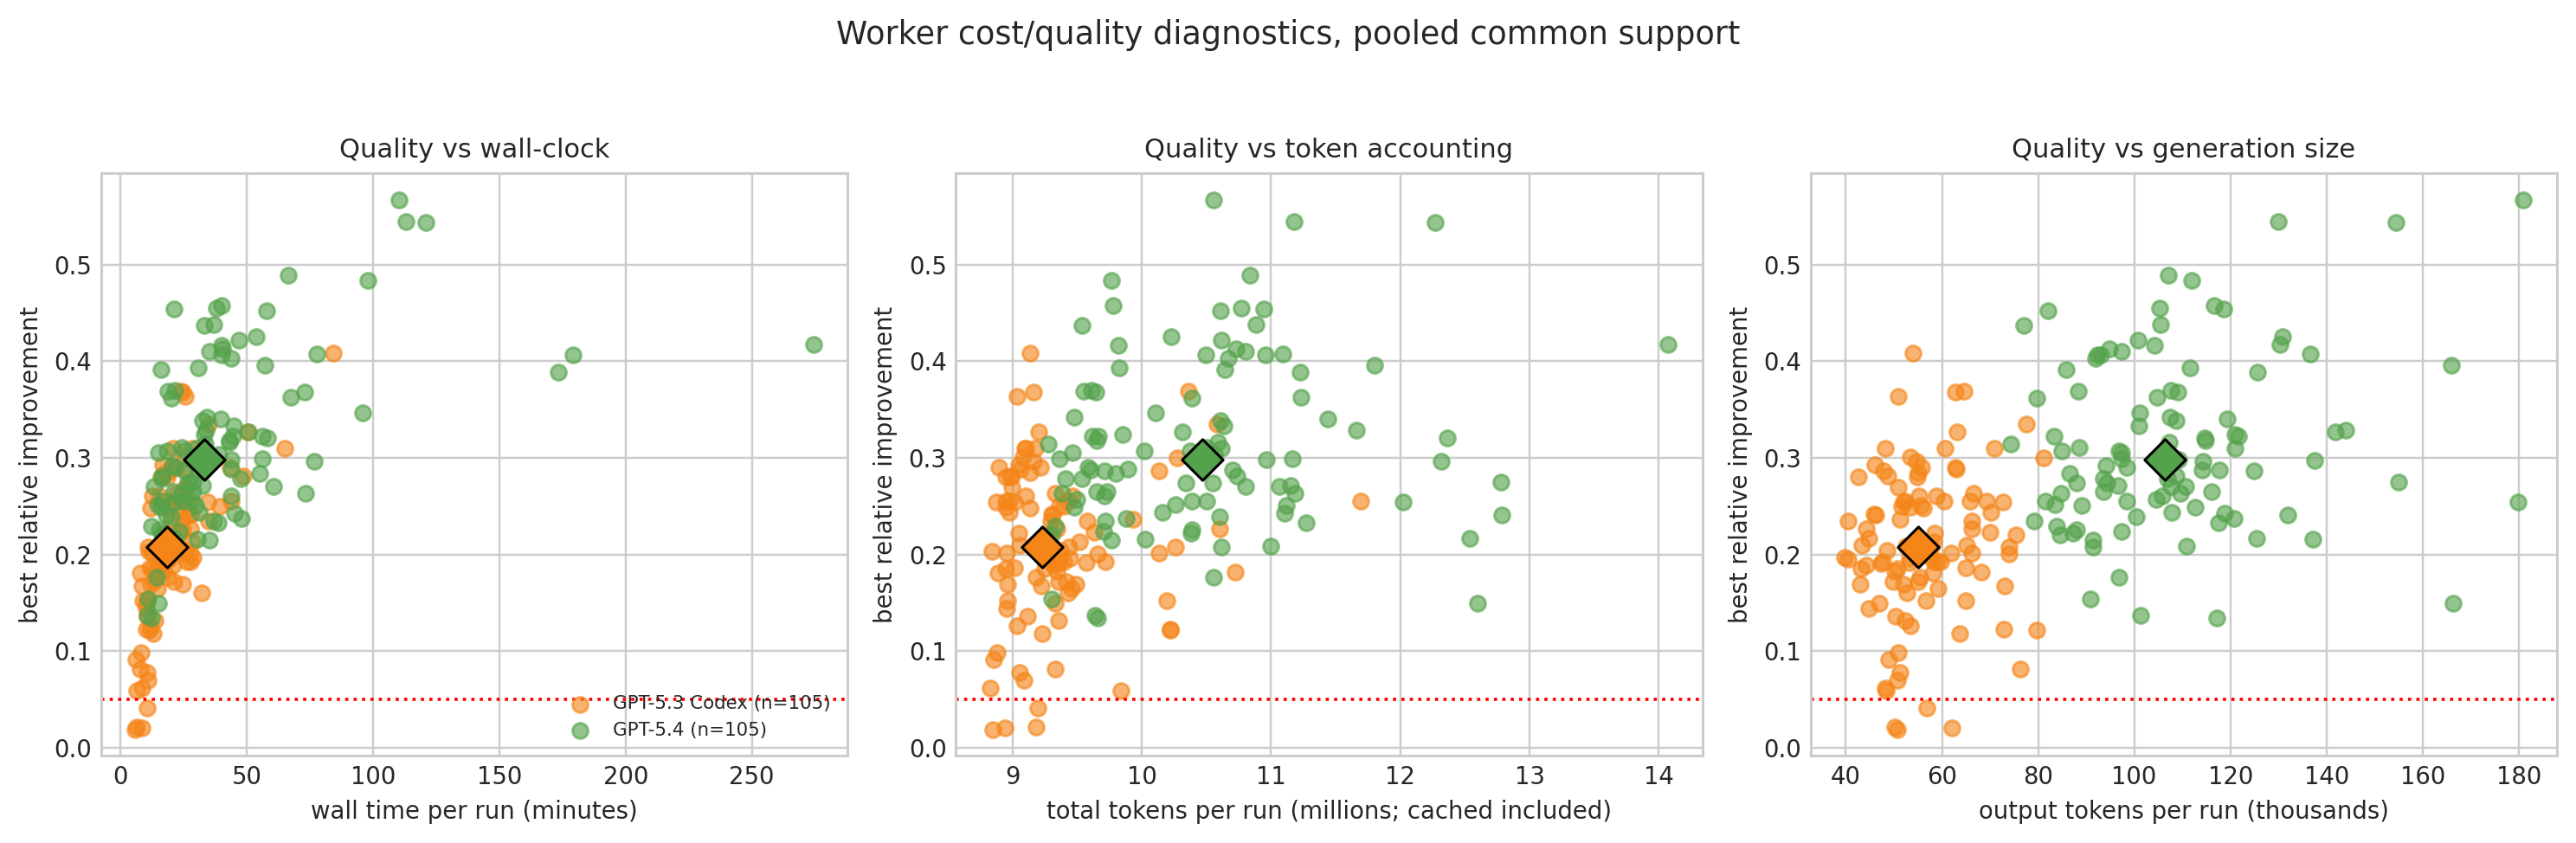
\includegraphics[width=\linewidth]{figures/autoresearch/diag_worker_cost_quality_diagnostics.png}
\caption{Worker cost--quality diagnostics.
Each point is a pooled common-support run, and diamonds mark worker medians.
The plots show that better final improvement is accompanied by substantial variation in wall-clock time, total token accounting, and generated-token volume.
This supports the paper's budget-aware framing: worker choice cannot be reduced to final improvement alone.}
\label{fig:app-worker-cost-quality-full}
\end{figure}

\begin{figure}[p]
\centering
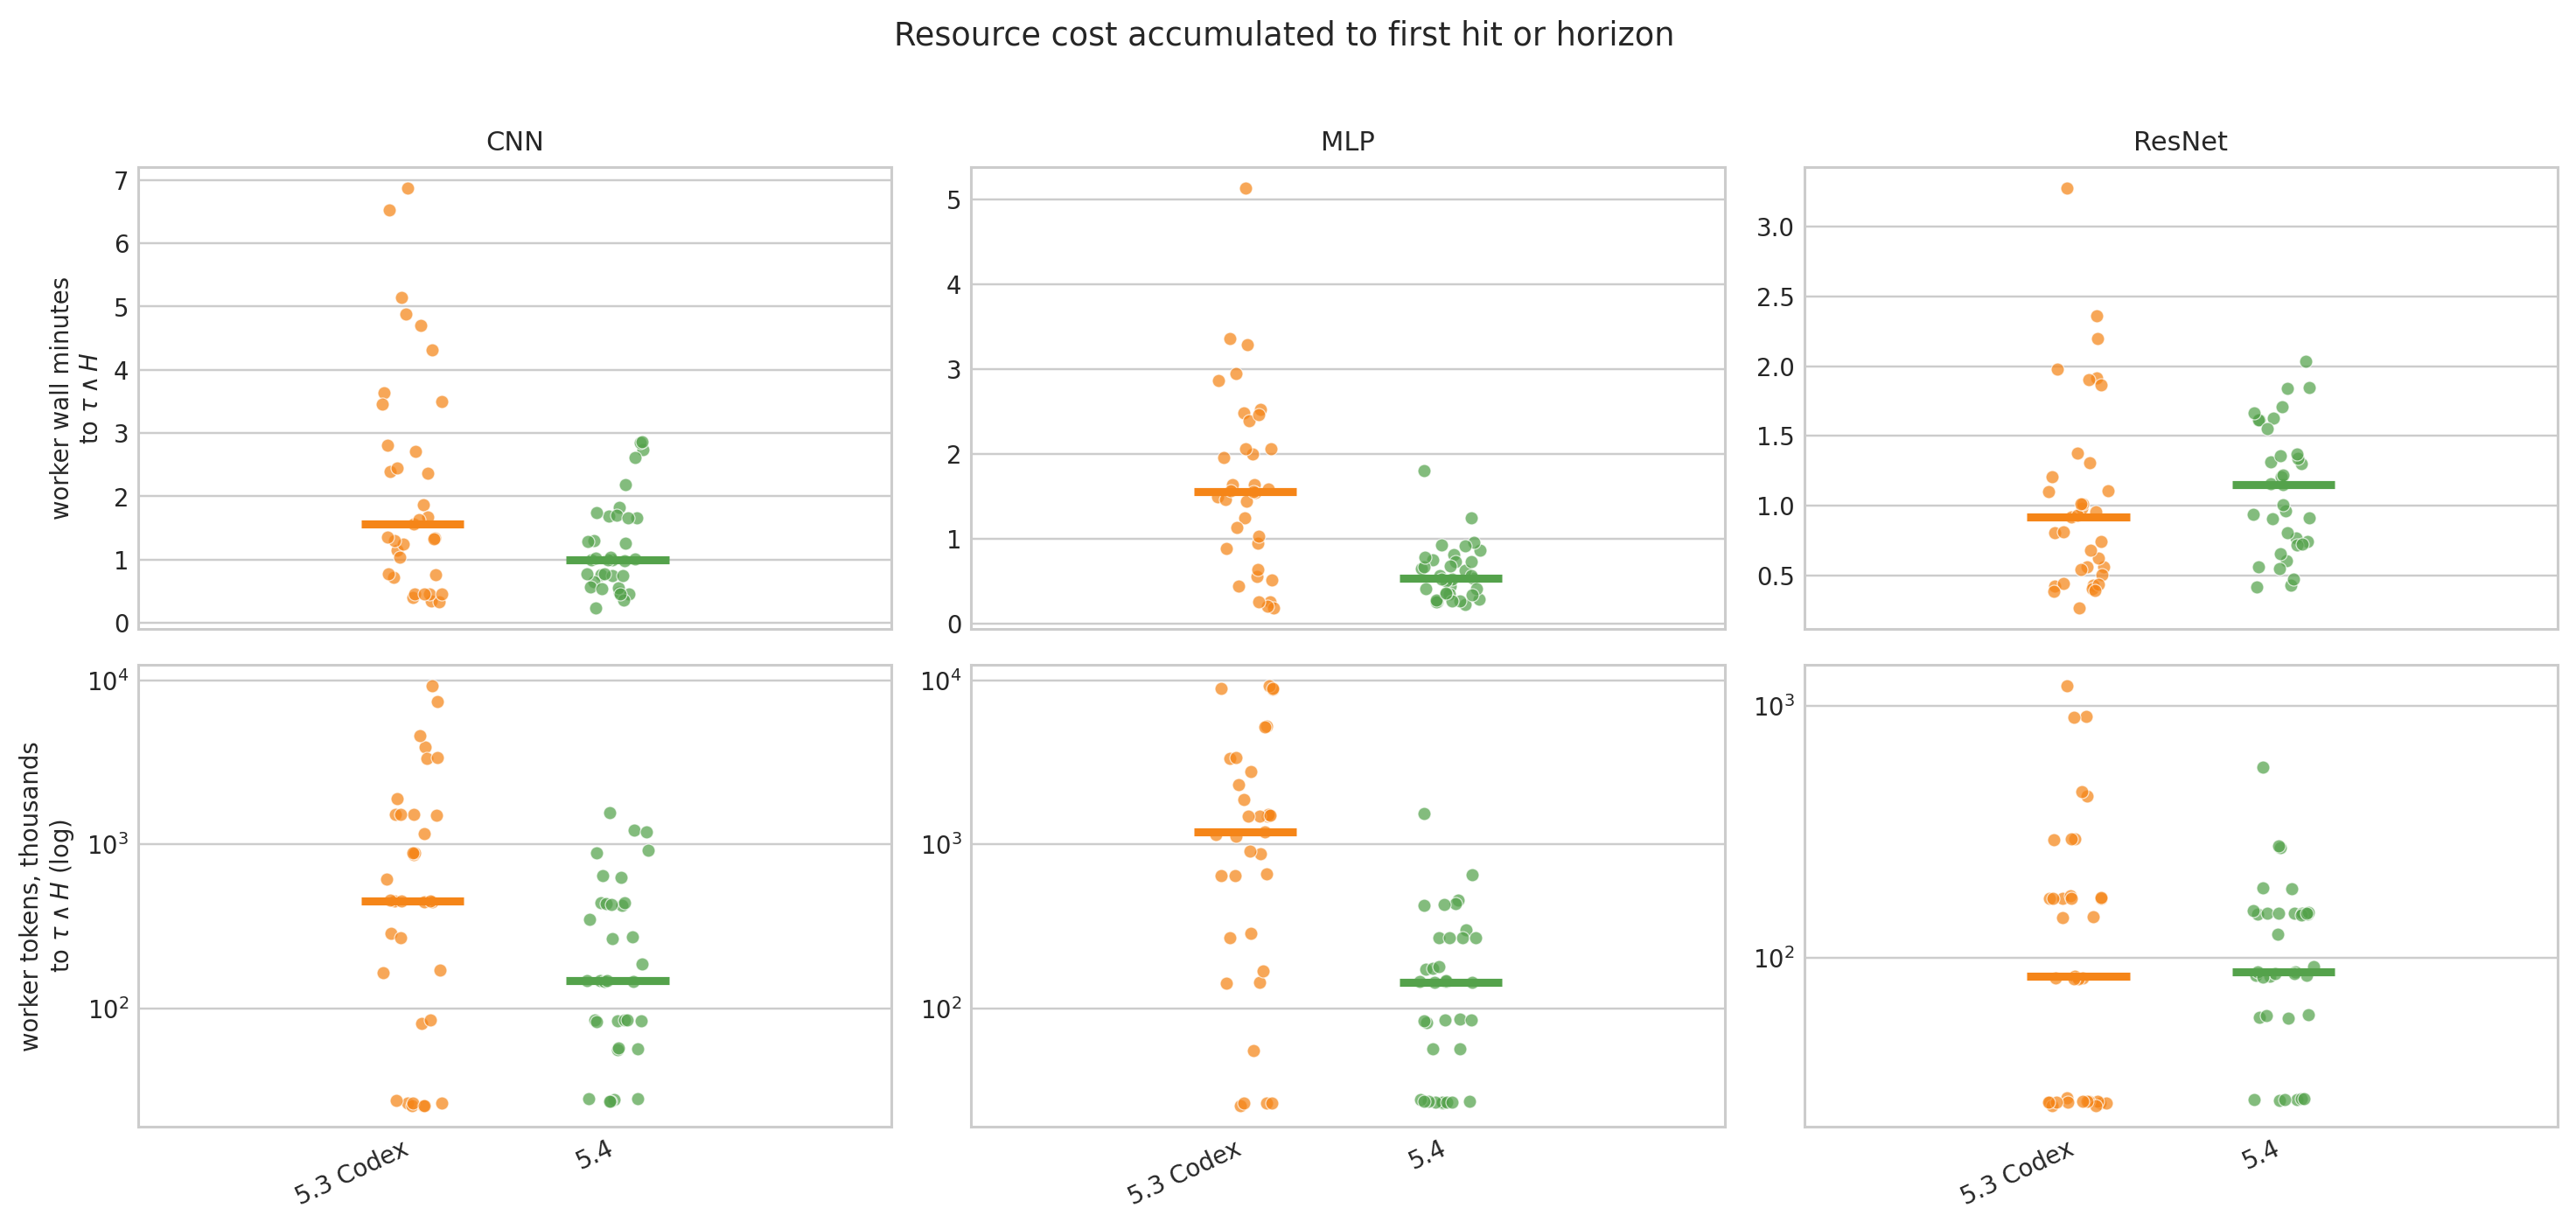
\includegraphics[width=\linewidth]{figures/autoresearch/diag_cost_to_tau_by_mode_worker_full.png}
\caption{Resource cost accumulated to first hit or horizon.
The top row reports wall-clock minutes and the bottom row reports token accounting on a log scale.
Mode-conditional cost spreads are large, which is why the retry-crossover theorem is treated as a cost-sensitive design rule rather than a generic endorsement of weaker workers.}
\label{fig:app-cost-to-tau-full}
\end{figure}

\begin{figure}[p]
\centering
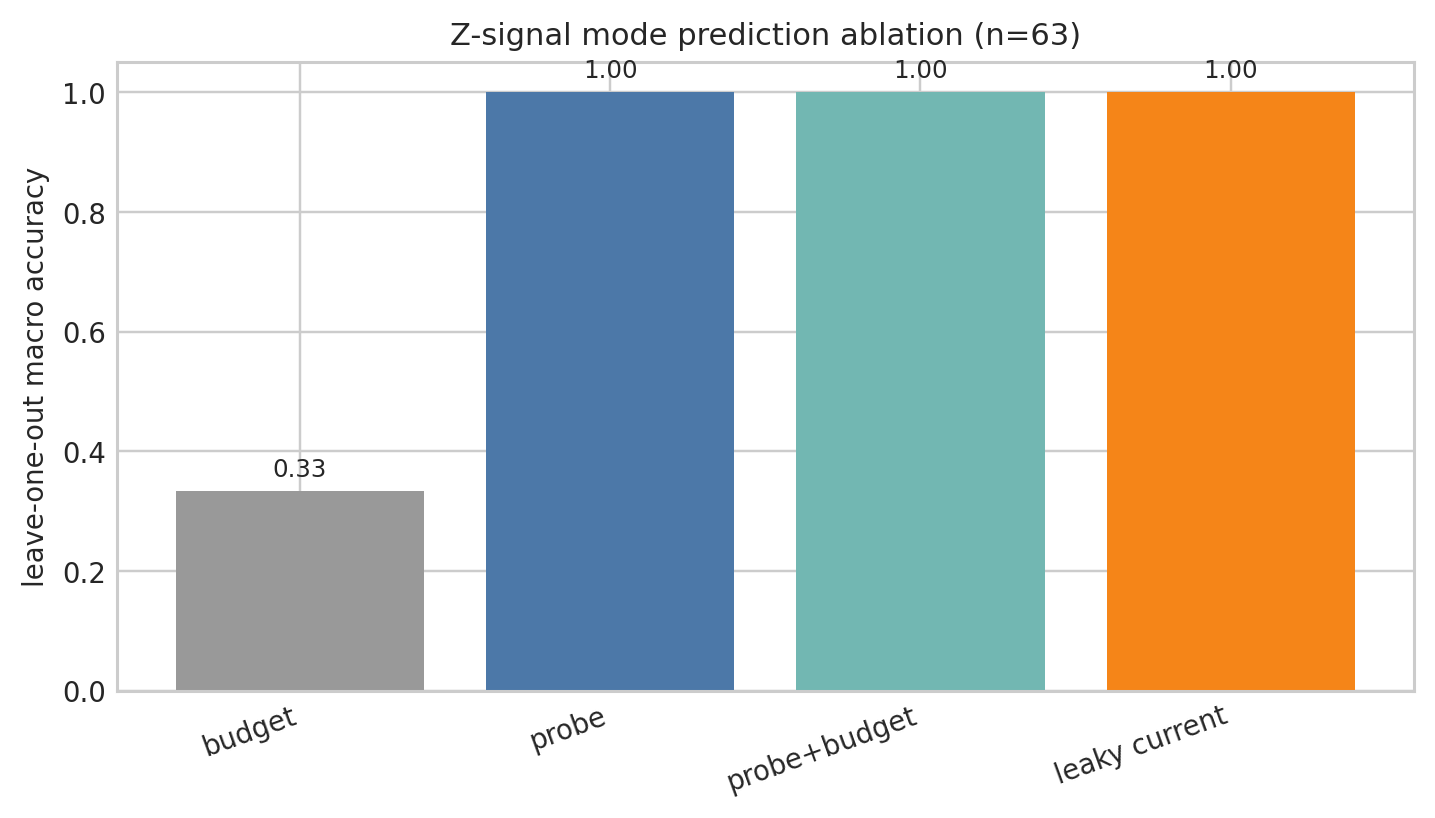
\includegraphics[width=0.92\linewidth]{figures/autoresearch/diag_z_signal_ablation.png}
\caption{Router-facing signal ablation.
The diagnostic tests whether progressively richer records expose the task-mode structure used in the accounting analysis.}
\label{fig:app-router}
\end{figure}

\clearpage
\section*{NeurIPS Paper Checklist}


\begin{enumerate}

\item {\bf Claims}
    \item[] Question: Do the main claims made in the abstract and introduction accurately reflect the paper's contributions and scope?
    \item[] Answer: \answerYes{}
    \item[] Justification: The abstract and introduction state the paper's scope: verifiable agentic systems, a packed latent-mode assumption, decomposition-guided selection, and a controlled fixed-prototype experimental protocol. The discussion section separates theory-facing and deployment-facing claims.
\item {\bf Limitations}
    \item[] Question: Does the paper discuss the limitations of the work performed by the authors?
    \item[] Answer: \answerYes{}
    \item[] Justification: Section~\ref{sec:discussion} discusses the packed-mode assumption, small live-agent sample sizes, finite design menus, oracle mode labels, and current cost-measurement limitations.
\item {\bf Theory assumptions and proofs}
    \item[] Question: For each theoretical result, does the paper provide the full set of assumptions and a complete (and correct) proof?
    \item[] Answer: \answerYes{}
    \item[] Justification: Assumption~\ref{ass:packed} states the assumptions for the main theoretical result, Theorem~\ref{thm:four-term} includes a proof sketch, and Appendix~\ref{app:proofs} gives the algebraic proof and pilot concentration details.
    \item {\bf Experimental result reproducibility}
    \item[] Question: Does the paper fully disclose all the information needed to reproduce the main experimental results of the paper to the extent that it affects the main claims and/or conclusions of the paper (regardless of whether the code and data are provided or not)?
    \item[] Answer: \answerYes{}
    \item[] Justification: Section~\ref{sec:experiments} describes the AutoResearch task instantiation, task modes, model menu, router-visible signals, horizons, metrics, and evaluation protocol; Appendix~\ref{app:experiment-details} specifies the required logs, estimators, and run-metadata fields.

\item {\bf Open access to data and code}
    \item[] Question: Does the paper provide open access to the data and code, with sufficient instructions to faithfully reproduce the main experimental results, as described in supplemental material?
    \item[] Answer: \answerNo{}
    \item[] Justification: The paper is written against an existing repository and includes reproducibility commands, but an anonymized public code/data release is not included in the current submission package.

\item {\bf Experimental setting/details}
    \item[] Question: Does the paper specify all the training and test details (e.g., data splits, hyperparameters, how they were chosen, type of optimizer) necessary to understand the results?
    \item[] Answer: \answerYes{}
    \item[] Justification: Section~\ref{sec:experiments} describes the AutoResearch task instantiation, task modes, model menu, router-visible signals, primary estimators, horizons, and evaluation design. Additional implementation details are listed in Appendix~\ref{app:experiment-details}.
\item {\bf Experiment statistical significance}
    \item[] Question: Does the paper report error bars suitably and correctly defined or other appropriate information about the statistical significance of the experiments?
    \item[] Answer: \answerYes{}
    \item[] Justification: Section~\ref{sec:experiments} and Appendix~\ref{app:experiment-details} specify Wilson intervals, bootstrap intervals, survival curves, calibration diagnostics, and held-out evaluation for the reported protocol.
\item {\bf Experiments compute resources}
    \item[] Question: For each experiment, does the paper provide sufficient information on the computer resources (type of compute workers, memory, time of execution) needed to reproduce the experiments?
    \item[] Answer: \answerNo{}
    \item[] Justification: The paper reports wall-clock costs and run counts but does not provide a complete compute-resource table for every experiment.
\item {\bf Code of ethics}
    \item[] Question: Does the research conducted in the paper conform, in every respect, with the NeurIPS Code of Ethics \url{https://neurips.cc/public/EthicsGuidelines}?
    \item[] Answer: \answerYes{}
    \item[] Justification: The work studies verifiable benchmark tasks and does not involve human subjects, sensitive personal data, or released high-risk models. The submission preserves anonymity and follows NeurIPS code and data policies.

\item {\bf Broader impacts}
    \item[] Question: Does the paper discuss both potential positive societal impacts and negative societal impacts of the work performed?
    \item[] Answer: \answerYes{}
    \item[] Justification: Section~\ref{sec:discussion} notes positive uses in cost-aware and transparent agent deployment as well as limitations and failure modes. The work is methodological and does not introduce a new generative model or dataset of people.
\item {\bf Safeguards}
    \item[] Question: Does the paper describe safeguards that have been put in place for responsible release of data or models that have a high risk for misuse (e.g., pre-trained language models, image generators, or scraped datasets)?
    \item[] Answer: \answerNA{}
    \item[] Justification: The paper does not release a pre-trained model, image generator, scraped dataset, or other asset with high misuse risk. It evaluates agent harnesses on synthetic or generated benchmark tasks.
\item {\bf Licenses for existing assets}
    \item[] Question: Are the creators or original owners of assets (e.g., code, data, models), used in the paper, properly credited and are the license and terms of use explicitly mentioned and properly respected?
    \item[] Answer: \answerYes{}
    \item[] Justification: The related-work section cites existing papers and systems used for positioning, and the experimental section describes the benchmark surfaces. Released code and benchmark assets include explicit license details.
\item {\bf New assets}
    \item[] Question: Are new assets introduced in the paper well documented and is the documentation provided alongside the assets?
    \item[] Answer: \answerYes{}
    \item[] Justification: The work introduces a code harness and analysis artifacts as research assets, and Appendix~\ref{app:experiment-details} documents the required logging and configuration fields.
\item {\bf Crowdsourcing and research with human subjects}
    \item[] Question: For crowdsourcing experiments and research with human subjects, does the paper include the full text of instructions given to participants and screenshots, if applicable, as well as details about compensation (if any)?
    \item[] Answer: \answerNA{}
    \item[] Justification: The paper does not involve crowdsourcing or research with human subjects.
\item {\bf Institutional review board (IRB) approvals or equivalent for research with human subjects}
    \item[] Question: Does the paper describe potential risks incurred by study participants, whether such risks were disclosed to the subjects, and whether Institutional Review Board (IRB) approvals (or an equivalent approval/review based on the requirements of your country or institution) were obtained?
    \item[] Answer: \answerNA{}
    \item[] Justification: The paper does not involve crowdsourcing or research with human subjects, so IRB or equivalent approval is not applicable.
\item {\bf Declaration of LLM usage}
    \item[] Question: Does the paper describe the usage of LLMs if it is an important, original, or non-standard component of the core methods in this research? Note that if the LLM is used only for writing, editing, or formatting purposes and does \emph{not} impact the core methodology, scientific rigor, or originality of the research, declaration is not required.
    %this research?
    \item[] Answer: \answerYes{}
    \item[] Justification: LLMs are central to the evaluated agent designs. Section~\ref{sec:experiments} describes the three-worker menu, fixed prompt-only router, sequential signal protocol, model-identifier logging, and routing-output requirements.
\end{enumerate}


\end{document}
